In his seminal paper \cite{STOC:Regev05}, Regev shows that the Learning with Errors problem (see Def.~\ref{def:LWE}) is at least as hard as certain hard lattice problems. It is thus important to understand how hard these lattices problems really are. This chapter addresses this question.

In more detail, we treat the Learning with Errors Problem as a Bounded Distance Decoding (\BDD) Problem on the lattice $\qLat(A\transpose)$: given $(\AMat, \tvec = \AMat\transpose \svec + \evec \bmod q) \in \Z_q^{n \times m} \times \Z_q^m$, we want to find the nearest to $\tvec$ lattice point $\AMat\transpose \svec \in \qLat(A\transpose)$. In other words, we want to solve a decoding problem for a code generated by $\AMat\transpose$ with messages from $\Z_q^n$ and codewords from $\Z_q^m$. The solution $\AMat\transpose \svec$ is unique since $\norm{\evec} \ll \lambda_1(\qLat(\AMat\transpose))$.  The error-vector $\evec$ is sampled from the discrete Gaussian distribution with parameter $\alpha q$ over the integer lattice $\Z_q^m$.

We start with the \emph{asymptotical} hardness of lattice-based decoding attacks on \LWE. In Sect.~\ref{sec:LWEasBDDAs}, we analyze the complexity of the problem under the following algorithms: Babai's $\NP$ Algorithm \cite{STACS:Babai85}, its extension due to Lindner and Peikert \cite{RSA:LinPei11}, and the Generalized Pruning Algorithm \GenPrun{}  -- a unification of the decoding strategies which allows us to analyze the existing lattice-based algorithms for \LWE/\BDD. The so-called Pruning algorithms of \cite{EC:GamNguReg10, RSA:LiuNgu13} appear as special cases of \GenPrun.

The main \LWE parameter that determines the complexity is the dimension of the secret -- $n$. All the aforementioned decoding algorithms are either super-exponential: $2^{\const n \log n + \smallo(n \log n)}$, or singe-exponential $2^{\const' n + \smallo(n)}$, where $\const, \const'$ are constants that depend on the other two \LWE parameters: $q, \alpha$. The goal of Sect.~\ref{sec:LWEasBDDAs} is to determine these constants $\const, \const'$. Note that from the modulus-dimension trade-off by Brakerski et al.\ \cite{STOC:BLPRS13}, stating that $\LWE$ preserves its hardness as long as the value $n\log q$ stays the same,  we can already explain why for all algorithms, the leading order constants $\const, \const'$ have a multiple of $\cq = \log q/ \log n$. 

The results of our analysis are summarized in Table~\ref{table:compareTable} in Sect.~\ref{subsec:Summary} where we list the running times of \emph{all} known attacks on \LWE together with constants in the exponents. These constants are made explicit as functions of the \LWE parameters $q, \alpha$. The table is translated into Fig.~\ref{fig:LWEPlots} to give a clear `winner' among all the known attacks for a concrete choice of \LWE parameters.

The second part is devoted to \emph{practical} hardness of \LWE. In Sect.~\ref{sec:LWEasBDDPr}, we present real running times of the Linear-Length Pruning attack on \LWE{} -- a pruning strategy that appears to perform best for the Learning with Errors problem.

The results of the first section are mainly based on \cite{DCC:HKM}. The cryptanalysis of real \LWE instances presented in Sect.~\ref{sec:LWEasBDDPr} is published in \cite{ACNS:KMW16}.

\section{Asymptotical Hardness of \LWE} \label{sec:LWEasBDDAs}
For a decoding algorithm $\ALG$, we will be interested in the quantity $\rho(\ALG) = \frac{T(\ALG)}{\Psucc(\ALG)}$, the trade-off between the running time and the success probability of $\ALG$ (in other words, we are interested in the expected time to decode successfully).  For an \LWE instance $(\AMat, \tvec = \AMat\transpose \svec + \evec \mod q)$, the decoding is successful if the returned lattice vector is indeed $\AMat\transpose \svec$ or, equivalently, the returned error is $\evec$. In the decoding algorithms we actually search for $\evec$.  It is easy to verify whether a given $\evec$ is correct or not, as the correct one is much shorter than an error-vector that leads to a wrong solution.

The algorithm we analyze here is a two-phase \BDD decoding algorithm: first, we preprocess a basis for $\qLat(\AMat\transpose)$ (given in Eq.~(\ref{eq:LWEBasis})) using $\beta$-\BKZ reduction to obtain a shorter basis. Denote this basis as $\BMat$. 
We do not explain here how the reduction works. 
All we need for the analysis is the running time of the reduction and the quality of its output. 
We use Eqs.~(\ref{eq:b1norm}) and (\ref{eq:GSA}) as guarantees on the quality of $\BMat$. 
Under these guarantees, during the second phase, we form a search space
to enumerate candidates for the error $\evec$ within this search space. The shortest candidate $\evec'$ is output as the solution.  We now explain how the actual decoding, i.e.\ enumeration, works.

Enumeration is done via orthogonal projection of the target vector $\tvec$ onto a (close) translate of the lattice $\Lat(\BMat)$: $i \bvec_m + \Span(\bvec_1, \ldots, \bvec_{m-1})$ for some appropriately chosen $i \in \Z$. A projected vector that now belongs to an $m-1$-dimensional $\Span(\bvec_1, \ldots, \bvec_{m-1})$ together with the lattice $\Lat(\bvec_1, \ldots, \bvec_{m-1})$ forms a new \BDD instance. We can run this procedure recursively. After $m$ such recursive projections, we end up with a lattice-vector (the last projection onto a zero-dimensional space is just choosing a close point) and hope it is the closest to the original $\tvec$.

The way we choose close translates on each recursive step defines the search space of the enumeration: restricting the search to the fundamental parallelepiped of the Gram-Schmidt basis of the lattice $\FP(\wBMat)$ gives Babai's $\NP$ algorithm \cite{STACS:Babai85}. 
Enlarging it by stretching $\FP(\wBMat)$ to a parallelepiped $ \FP(\wBMat \cdot \DMat)$ for some diagonal matrix $\DMat$ results in the Linder-Peikert $\NPs$ algorithm \cite{RSA:LinPei11}.
Considering error-vectors $\evec$ that lie within some ball of radius $R$ gives rise to the Spherical Pruning \cite{SchE94}.
The so-called Linear-Length pruning of \cite{EC:GamNguReg10} forms a search space of cylinder intersections (i.e.\ a candidate error-vector $\evec$ is enumerated if its coordinates satisfy the system of inequalities $\{e_1^2 \leq R_1, e_1^2 + e_2^2 \leq R_2, \ldots, \| \evec \|^2 \leq R_n \}$ for some input-sequence $R_1, \ldots, R_n$).

Certainly, one is free to choose a search space of any shape and hope it will bring an improvement to the enumeration phase. By `improvement' we mean a better running-time/success probability trade-off $\rho$. We notice that the aforementioned pruning strategies share some common `rules', which allows us to analyze them at one shot.  To do that we define what we call a \emph{reasonable} pruning strategy that describes these `rules', give the algorithm $\GenPrun$ that follows this strategy, and analyze its complexity. It turns out that the Spherical Pruning, Linear-Length Pruning and other (called `Extreme' in \cite{EC:GamNguReg10}) pruning strategies are all reasonable, so it is sufficient to consider our generalization to conclude on their asymptotics.

To achieve our original goal -- to determine the complexity of \LWE as a \BDD problem -- we show in Sects.~\ref{sec:BabaisNP} -- \ref{sec:GenPrun} the running time/success probability trade-off $\rho(\ENUM) = \frac{T(\ENUM)}{\Psucc(\ENUM)}$, where we consider $\ENUM \in\{ \text{Babai's } \NP, \allowbreak \text{Lindner-Peikert's } \NPs, \GenPrun \}$. Since $\ENUM$ is only the second step of the whole algorithm, the actual trade-off on the \BDD attack is $\rho(\BDD) = \frac{T(\BKZ) + T(\ENUM)}{\Psucc(\ENUM)}$. We take care about it in Sect.~\ref{sec:Balance}.

\subsection{Babai's $\NP$ Algorithm} \label{sec:BabaisNP}

Suppose we are given a lattice-basis $\BMat = (\bvec_1, \ldots, \bvec_m) \in \Z^{m \times m}$ and a target point $\tvec \in \Q^m$.\footnote{While for $\LWE$ the target and the lattice agree in the dimension, this is not required for the algorithm to work. If they do not agree, we project $\tvec$ onto $\Span(\Lat(\BMat))$  and work with the projection as the input target.} 
We search for a lattice-vector $\vvec \in \Lat(\BMat)$ that is close to $\tvec$.
Babai's algorithm works as follows. We view the $m$-dimensional lattice $\Lat(\BMat)$ as the $m-1$-dimensional lattice $\Lat(\bvec_1, \ldots, \bvec_{m-1})$ translated via shifts $i \bvec_m$:
\[
 \Lat(\BMat) = \bigcup_{i \in \Z} i \bvec_m + \Lat(\bvec_1, \ldots, \bvec_{m-1}).
\]
Fixing $i$, we receive a translate $i \bvec_m + \Lat(\bvec_1, \ldots, \bvec_{m-1}) \subset U_i^{(m-1)}$ that is contained in the $m-1$-dimensional hyperplane $U_i^{(m-1)} = \bigl\{\yvec \in \R^m \colon \bigScProd{\yvec}{\frac{\wbvec_m}{\| \wbvec_m \|^2}} = i \bigr\}$ (cf.\ Fig.~\ref{fig:NP1}).
Babai's algorithm chooses a hyperplane $U_i^{(m-1)}$ that is closest to $\tvec$ (see line \ref{algline:BabaiChoosePlane} in Alg.~\ref{alg:Babai}) with the corresponding translate $\xvec^{(m)} = i \bvec_m$ (line \ref{algline:BabaiChooseTranslate}), and then projects $\tvec = \tvec^{(m)}$ orthogonally onto $U_i^{(m-1)}$ to obtain $\tvec^{(m-1)}$ (line \ref{algline:BabaiProjectTarget}). 

Now we have a new target $\tvec^{(m-1)}$ and a (shifted) sub-lattice $\xvec^{(m)} + \Lat(\bvec_1, \ldots, \bvec_{m-1})$, so we repeat the process by choosing $U_j^{(m-2)} = \smash{ \bigl\{\yvec \in \R^m \colon \bigScProd{\yvec}{\frac{\wbvec_{m-1}}{\| \wbvec_{m-1} \|^2}} = j +  \bigScProd{\xvec^{(m)}}{\frac{\wbvec_{m-1}}{\| \wbvec_{m-1} \|^2}} \text{ and } \bigScProd{\yvec}{\frac{\wbvec_m}{\| \wbvec_m \|^2}} = i \bigr\} }$ closest to $\tvec^{(m-1)}$ (note that $U_j^{(m-2)} \subset U_i^{(m-1)}$). The shifts $\xvec^{(k)}$  accumulate the output vector $\vvec$ coordinate-wise w.r.t.\ the basis $\BMat$ starting from $\bvec_m$. In the algorithm described below, we also keep track of the error incurred by projections. The output error vector $\evec'$ is constructed coordinate-wise w.r.t.\ the Gram-Schmidt basis $\wBMat$ starting from $\wbvec_m$.
%
% BABAI's algorithm
%
\setlength{\intextsep}{\medskipamount}
\begin{algorithm}[h]
\caption{Babai's $\NP$ $(\BMat, \xvec, \protect \tvec)$}
\label{alg:Babai}
\textbf{Input:} $\BMat=(\bvec_1, \ldots, \bvec_m) \in \Z^{m \times m}, \xvec \in \Q^m, \tvec \in \xvec+\Span(\BMat), \evec' \in \Q^m$ \hfill \Comment \scriptsize{$\evec'=\xvec=0, k=m$ in the initial call}\\
\normalsize
\textbf{Output:} $\vvec\in \Lat(\BMat)$ close to $\tvec$ and $\evec' = \tvec-\vvec$ corresponding error vector
\begin{algorithmic}[1]
\State $\xvec^{(k)}\gets \xvec, \tvec^{(k)}\gets \tvec,\evec'^{(k)}\gets\evec'$. 
\State Let $\wBMat \gets \GSO(\BMat)$. 
\If {$k=0$} \Return $(\xvec,\evec')$
\EndIf
\State Compute $c^{(k)}_1 \gets \bigScProd{\tvec^{(k)}}{\frac{\wbvec_k}{ \vphantom{\scalebox{1.6}x^2} \|\wbvec_k \|^2}}$
\State Choose $i^{(k)} \in \Z$ s.t.\ $c^{(k)}_2 = \bigScProd{\xvec^{(k)}}{\frac{\wbvec_k}{\|\wbvec_k \|^2}} + i^{(k)}$ closest to $c^{(k)}_1$ \label{algline:BabaiChoosePlane}
\State $\xvec^{(k-1)}\gets \xvec^{(k)}+i^{(k)}\bvec_k$ \label{algline:BabaiChooseTranslate}
\Comment $U_i^{(k-1)} = \xvec^{(k-1)}+\Lat(\BMat^{(k-1)})$ is the nearest plane
\State $\evec'^{(k-1)}\gets \evec'^{(k)} + (c^{(k)}_1-c^{(k)}_2)\wbvec_k$
\State $\tvec^{(k-1)}=\tvec^{(k)} - (c^{(k)}_1-c^{(k)}_2)\wbvec_k$ \label{algline:BabaiProjectTarget} \Comment Project onto $U_i^{(k-1)}$ 
\State \Return $\texttt{NearestPlanes} ((\bvec_1,\ldots,\bvec_{k-1}), \xvec^{(k-1)},\tvec^{(k-1)},\evec'^{(k-1)})$
\end{algorithmic} 
\end{algorithm}

\paragraph{Analysis.} It is easy to verify that Babai's Algorithm runs in time polynomial in $m$. In the context of \LWE, the algorithm succeeds (i.e.\ the output vector $\evec'$ is the \LWE error $\evec$) if $\evec$ lies in the interior of $\FP(\wBMat)$. In other words, if we write $\evec = \sum_k e_k \frac{\wbvec_k}{ \| \wbvec_k \|}$ w.r.t.\ the normalized Gram-Schmidt basis, we have $\evec = \evec'$ if $\abs{e_k} < \tfrac{1}{2} \|\wbvec_k \|$. If there exist an index $k$ s.t.\ $\abs{e_k} > \tfrac{1}{2} \|\wbvec_k \|$, the algorithm fails. In case, $\abs{e_k} = \tfrac{1}{2} \|\wbvec_k \|$, there will be two equally close translates and we choose one arbitrarily. This case does not affect the asymptotics.

For the analysis, we approximate the discrete Gaussian $\evec$ by a continuous one, i.e., the $e_k$'s are assumed to be independent Gaussians with parameter $\alpha q$. Note that expressing $\evec$ in terms of the normalized Gram-Schmidt basis (instead of the standard $\Z$-basis) does not change the distribution of $e_k$ as the former basis is just a rotation of the later one and the continuous Gaussian distribution is rotation-invariant. 

Recall that Babai's algorithm receives as input a $\beta$-\BKZ reduced basis $\BMat$. Under the Geometric Series Assumption (Eq.~(\ref{eq:GSA})), the sequence $\| \wbvec_1 \|, \ldots, \| \wbvec_m\|$ decays geometrically. Combining this with the guarantee on $\| \bvec_1\|$ (Eq.~(\ref{eq:b1norm})), we can say whether (1) $\| \wbvec_m\|> \alpha q$ (and the success probability of the algorithm is constant), or (2) $\| \wbvec_1 \| = \alpha q$ (the success probability is super-exponentially low). In the intermediate case (relevant for our \LWE setting), $ \| \wbvec_m \| \ll \alpha q \ll \| \wbvec_1 \|$, all the steps $k$ for which $\| \wbvec_k \| \ll \alpha q $ contribute to a super-exponentially small success probability, while the steps starting from $\| \wbvec_j \| \approx \alpha q$ do not change the success probability much. The next lemma formalizes these arguments.

\begin{lemma} \label{lem:BabaiHelpingLemma}
Let the sequence $\|\wbvec_1 \|, \ldots, \|\wbvec_m \|$ be geometrically decreasing with $\|\wbvec_k \| / \|\wbvec_{k+1} \| = \beta^{1/ \beta} >1$. Let $e_1, \ldots, e_m$ be independent continuous Gaussians with the density function $\varrho(x) = \tfrac{1}{s} \exp(-\frac{\pi x^2}{s^2})$. Denote $p_k := \Pr[ \abs{e_k} < \| \wbvec_k \|]$.
	\begin{enumerate}
		\item If $\| \wbvec_m \| > s (\log{m})^{1/2 + \eps}$ for fixed constant $\eps>0$, then $\prod_k p_k = 1 - \smallo(1)$.
		\item If $\| \wbvec_1 \| = s$, then $\prod_k p_k = 2^{-\bigO(m)} \cdot 2^m \beta^{-\frac{1}{2} \frac{m(m+1)}{\beta}}$.
	\end{enumerate}
\end{lemma}  

\begin{proof}
	To see the first statement, we use the Gaussian tails-bounds Eq.~(\ref{eq:TailBound}). For $\| \bvec_k \| > s (\log{m})^{1/2 + \eps}$, $1-p_k$ is super-polynomially small, namely, $1-p_k = e^{-\TLandau((\log{m})^{1+2\eps})}$. The result follows from the union bound and the fact that $e^{-t} \sim 1-t$ for $t \rightarrow 0$. 
	
	For the second statement, informally, we approximate the area under the Bell-shaped curve on the interval $[- \| \wbvec_i \|, \| \wbvec_k \|]$ with a parallelepiped. More precisely,
	\[
		p_k = \frac{1}{2 \varrho_s(\Z)}\int\limits_{- \| \wbvec_k \|}^{ \| \wbvec_k \|} \exp \Bigl(-\frac{\pi x^2}{s^2} \Bigr) \d x = \TLandau(1) \frac{2 \| \wbvec_k \|}{s}.
	\]
Then 
	\[
		\prod_k p_k = 2^{-\bigO(n)} \cdot 2^n \frac{ \prod_k \| \wbvec_k \|}{s^n} = 2^{-\bigO(m)} \cdot 2^n  \frac{\|\wbvec_1\|^m}{s^m} \prod_{i=2}^{m} \beta^{-i/ \beta} = 2^{-\bigO(m)} \cdot 2^m \beta^{-\frac{1}{2} \frac{m(m+1)}{\beta}}. 
	\]
\end{proof}

For $\LWE$, we have $s = \alpha q$. Recall that we relate the \LWE parameters $(n, q, \alpha)$ as $q = \bigO(n^{\cq})$, $\alpha~= \bigO(1 / n^{\ca})$ for positive constants $\cq, \ca $, $\cq > \ca$, from where it easily follows that the width $s=\alpha q$ is $ \bigO(n^{\cq-\ca})$. With the above lemma, we show the the success probability of Babai's algorithm depends on whether $\|\wbvec_m \|$ is larger or smaller than $s = \alpha q$. %The number of \LWE samples $m$ is linear in $n$. 

\begin{thm}[Analysis of the $\NP$ Algorithm~\ref{alg:Babai}] \label{thm:PsuccBabai}
	Given a $\beta = \TLandau(n)$-\BKZ reduced basis that arises from $m = \TLandau(n)$ \LWE-samples with parameters $(n, q=\bigO(n^{\cq}), \alpha = \bigO(1 / n^{\ca}) )$ for positive constants $\cq>\ca$, Babai's $\NP$ Algorithm~\ref{alg:Babai} solves the Search-\LWE problem in time $\poly(m)$ with success probability
	\begin{equation*}
\Psucc(\NP)=\begin{cases}
                  2^{-\frac{1}{2} \bigl(\frac{m}{2\beta}-\ca + \frac{n}{m} \cq  \bigr)^2 (1+\smallo(1)) \cdot \beta\log\beta},			      \quad & \text{if }  \frac{m}{2 \beta} - \ca + \frac{n}{m} \cq  > 0  \\
                  1-o(1),                                     \quad&\text{if } \frac{m}{2 \beta} - \ca + \frac{n}{m}\cq  < 0,
                  \end{cases}
\end{equation*}
assuming the Geometric Series Assumption holds and the \LWE error follows a continuous Gaussian distribution.
\end{thm}

\begin{proof}
	From Eqs.~(\ref{eq:GSA}), (\ref{eq:b1norm}), we have $\| \wbvec_i \| = \beta^{\frac{m}{2 \beta} - \frac{i}{\beta}} \cdot q^{1 - \frac{n}{m}}$. We want to compute a `critical' level $k^*$ s.t.\ $\| \wbvec_{k^*} \| = \alpha q$. It is easy to verify that $k^* = \beta \bigl( \frac{m}{2 \beta} - \frac{n}{m} \cq + \ca \bigr)$, from where it follows
	\begin{equation} \label{eq:BabaiProof}
		m - k^* = \beta \Bigl( \frac{m}{2 \beta} + \frac{n}{m} \cq - \ca \Bigr).
	\end{equation}
In case $\frac{m}{2 \beta} + \frac{n}{m} \cq - \ca < 0$, we have $m < k^*$ and $\| \wbvec_m \| > \alpha q \cdot \poly(n)$. So all the Gram-Schmidt vectors are large enough to guarantee a super-polynomially small (in $m$) error probability on each level. From Lemma~\ref{lem:BabaiHelpingLemma}, first statement, the success probability of Algorithm~\ref{alg:Babai} is then $1-\smallo(1)$.

In case $\frac{m}{2 \beta} + \frac{n}{m} \cq - \ca > 0$, we use the second statement of Lemma~\ref{lem:BabaiHelpingLemma} having $\| \wbvec_{k^*} \| = \alpha q$ instead of $\| \wbvec_1\|$ and obtain
	\[
		\Psucc(\NP) = 2^{-\bigO(m-k^*)} \cdot 2^{m-k^*} \beta^{-\frac{1}{2} \frac{(m-k^*)^2}{\beta}} = 2^{-\frac{1}{2} \bigl(\frac{m}{2\beta}-\ca + \frac{n}{m} \cq  + \smallo(1) \bigr) ^2 \cdot \beta \log\beta}.
	\]
\end{proof}

\subsection{Lindner-Peikert \NPs Algorithm} \label{sec:LPNP}
\begin{figure}
	\begin{subfigure}[b]{0.32\textwidth}
	\centering
	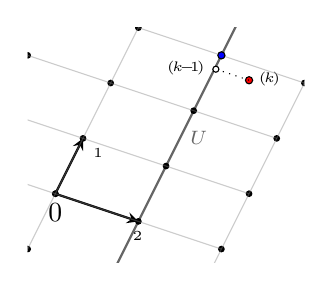
\begin{tikzpicture}
		\clip (-10pt,-25pt) rectangle (90pt, 60pt);
			%\draw[step=10pt,gray,opacity=0.1, very thin] (-40pt,-30pt) grid (100pt, 100pt);
			\foreach \y in {-2,...,5}
			\foreach \x in {-2,...,3}
			\filldraw(\x*40pt+\y*10pt, 10pt*\x+20pt*\y) circle (1pt);
			\filldraw(0pt,0pt) circle (1pt) node[below]{$0$};

			\draw[->, -stealth, black, thick] (0,0) -- (30pt, -10pt) node[font=\tiny, below]{$\bvec_2$};
			\draw[->, -stealth, black, thick] (0,0) -- (10pt, 20pt) node[font=\tiny, below right]{$\bvec_1$};
			\filldraw[fill=red](70pt, 41pt) circle (1.3pt) node[font=\tiny, right]{$\tvec^{(\mkern-2mu k \mkern-2mu)}$};
			%vertical lines:
			%\draw[gray, opacity=0.4] (-40pt, -10pt) -- (0pt, 70pt);
			\draw[gray, opacity=0.4] (-20pt, -40pt) -- (40pt, 80pt);
			\draw[black, thick, opacity=0.6] (20pt, -30pt) -- (70pt, 70pt) node[font=\scriptsize, midway, right]{$U$};
			\draw[gray, opacity=0.4] (50pt, -40pt) -- (90pt, 40pt);

			%horizontal lines:
			\draw[gray, opacity=0.4] (-30pt, 10pt) -- (60pt, -20pt);
			\draw[gray, opacity=0.4] (-20pt, 30pt) -- (70pt, 0pt);
			\draw[gray, opacity=0.4] (-40pt, 60pt) -- (80pt, 20pt);
			\draw[gray, opacity=0.4] (30pt, 60pt) -- (90pt, 40pt);
			%\draw[gray, opacity=0.4] (-50pt, -30pt) -- (70pt, 0pt);	
			
			%projection
			\draw[black, dotted] (70pt, 41pt) -- (58pt, 45pt);
			\filldraw[fill=white](58pt, 45pt) circle (1.1pt) node[font=\tiny, left] {$\tvec^{(\mkern-2mu k\mkern-3mu - \mkern-4mu 1 \mkern-2mu)}$};
			
			%solution
			\filldraw[fill=blue](60pt, 50pt) circle (1.3pt) node[font=\tiny, right]{$\vvec$};
	\end{tikzpicture}
	\caption{\scriptsize Babai's $\NP$ Algorithm on a `good' basis. The target point $t^{(k)}$ (red) is projected onto the closest hyperplane $U=\bvec_2+\Span(\bvec_1).$ The recursive call for this 1-dimensional $U$ projects $\tvec^{(k-1)}$ onto the closest zero-dimensional subspace, i.e.\ lattice point $\vvec$ (blue). }
                \label{fig:NP1}
	\end{subfigure}%
	~
    \begin{subfigure}[b]{0.32\textwidth}
    		\centering
    		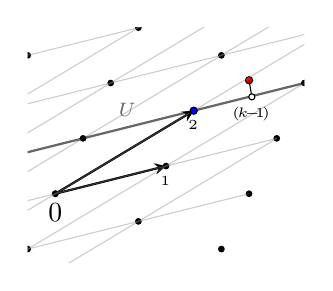
\begin{tikzpicture}
		\clip (-10pt,-25pt) rectangle (90pt, 60pt);
			\foreach \y in {-2,...,5}
			\foreach \x in {-2,...,3}
			\filldraw(\x*40pt+\y*10pt, 10pt*\x+20pt*\y) circle (1pt);
			\filldraw(0pt,0pt) circle (1pt) node[below]{ $0$};

			\draw[->, -stealth, black, thick] (0,0) -- (40pt, 10pt) node[font=\tiny, below]{$\bvec_1$};
			\draw[->, -stealth, black, thick] (0,0) -- (50pt, 30pt) node[font=\tiny, below]{$\bvec_2$};
			\filldraw[fill=red](70pt, 41pt) circle (1.3pt) node[font=\tiny, right]{$\tvec$};
			%vertical lines:
			\draw[gray, opacity=0.4] (-50pt, -30pt) -- (100pt, 60pt);
			\draw[gray, opacity=0.4] (-40pt, -10pt) -- (110pt, 80pt);
			\draw[gray, opacity=0.4] (-30pt, 10pt) -- (70pt, 70pt);
			\draw[gray, opacity=0.4] (-70pt, 0pt) -- (80pt, 90pt);
			\draw[gray, opacity=0.4] (-60pt, -50pt) -- (90pt, 40pt);
			\draw[gray, opacity=0.4] (-20pt, -40pt) -- (80pt, 20pt);
			
			%horizontal lines:
			\draw[gray, opacity=0.4] (-50pt, 40pt) -- (70pt, 70pt);
			\draw[gray, opacity=0.4] (-60pt, 20pt) -- (100pt, 60pt);
			\draw[black, thick, opacity=0.6] (-70pt, 0pt) -- (90pt, 40pt) node[font=\scriptsize, above, pos=0.6]{$U$};
			\draw[gray, opacity=0.4] (-40pt, -10pt) -- (80pt, 20pt);
			\draw[gray, opacity=0.4] (-50pt, -30pt) -- (70pt, 0pt);	
			
			%projection 
			\draw[black] (70pt, 41pt) -- (71pt, 35pt);
			\filldraw[fill=white](71pt, 35pt) circle (1.1pt) node[font=\tiny, below] {$\tvec^{(\mkern-2mu k\mkern-3mu - \mkern-4mu 1 \mkern-2mu)}$};
			
			%solution
			\filldraw[fill=blue](50pt, 30pt) circle (1.3pt) node[font=\tiny, left, above]{$\vvec$};
			
	\end{tikzpicture}
	\caption{\scriptsize Babai's $\NP$ Algorithm on a `bad' basis for the same lattice. Now the target point $\tvec^{(k)}$ (red) is projected onto the hyperplane $U=\bvec_2+\Span(\bvec_1)$ but for different $\bvec_2, \bvec_1$, so the hyperplane has changed. The returned vector $\vvec$  is not the closest vector.}
	\label{fig:NP2}
    \end{subfigure}%
    ~
    \begin{subfigure}[b]{0.32\textwidth}
    		\centering
    		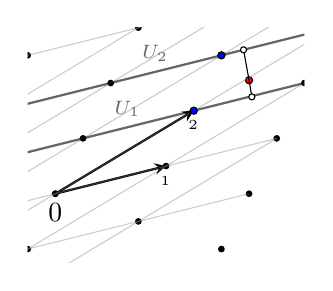
\begin{tikzpicture}
		\clip (-10pt,-25pt) rectangle (90pt, 60pt);
			%\draw[step=10pt,gray,opacity=0.1, very thin] (-40pt,-30pt) grid (100pt, 100pt);
			\foreach \y in {-2,...,5}
			\foreach \x in {-2,...,3}
			\filldraw(\x*40pt+\y*10pt, 10pt*\x+20pt*\y) circle (1pt);
			\filldraw(0pt,0pt) circle (1pt) node[below]{ $0$};

			\draw[->, black, -stealth, thick] (0,0) -- (40pt, 10pt) node[font=\tiny, below]{$\bvec_1$};
			\draw[->, black, -stealth, thick] (0,0) -- (50pt, 30pt) node[font=\tiny, below]{$\bvec_2$};
			\filldraw[fill=red](70pt, 41pt) circle (1.3pt) node[font=\tiny, right]{$\tvec$};
			%vertical lines:
			\draw[gray, opacity=0.4] (-50pt, -30pt) -- (100pt, 60pt);
			\draw[gray, opacity=0.4] (-40pt, -10pt) -- (110pt, 80pt);
			\draw[gray, opacity=0.4] (-30pt, 10pt) -- (70pt, 70pt);
			\draw[gray, opacity=0.4] (-70pt, 0pt) -- (80pt, 90pt);
			\draw[gray, opacity=0.4] (-60pt, -50pt) -- (90pt, 40pt);
			\draw[gray, opacity=0.4] (-20pt, -40pt) -- (80pt, 20pt);
			
			%horizontal lines:
			\draw[gray, opacity=0.4] (-50pt, 40pt) -- (70pt, 70pt);
			\draw[black, thick, opacity=0.6] (-60pt, 20pt) -- (100pt, 60pt) node[font=\scriptsize, above, pos=0.6]{$U_2$};
			\draw[black, thick, opacity=0.6] (-70pt, 0pt) -- (90pt, 40pt) node[font=\scriptsize, above, pos=0.6]{$U_1$};
			\draw[gray, opacity=0.4] (-40pt, -10pt) -- (80pt, 20pt);
			\draw[gray, opacity=0.4] (-50pt, -30pt) -- (70pt, 0pt);	
			
			%projections 
			\draw[black] (70pt, 41pt) -- (71pt, 35pt);
			\filldraw[fill=white](71pt, 35pt) circle (1.1pt);
			
			\draw[black] (70pt, 41pt) -- (68pt, 52pt);
			\filldraw[fill=white](68pt, 52pt) circle (1.1pt);
			
			%solutions
			\filldraw[fill=blue](50pt, 30pt) circle (1.3pt);
			\filldraw[fill=blue](60pt, 50pt) circle (1.3pt) node[font=\tiny, above]{$\vvec$};
	\end{tikzpicture}
	\caption{\scriptsize Lindner-Peikert $\NPs$ Algorithm on the same `bad' basis. We set $\dvec = (1, 2)$ and project the target $\tvec$ onto two hyperplanes $U_1 = \bvec_2+\Span(\bvec_1), U_2 = 2\bvec_2+\Span(\bvec_1)$. The output points are marked blue. The closets point $\vvec$ is found among them.}
	\label{fig:NP3}
    \end{subfigure}%
    \caption{$\NP$(\texttt{s}) Algorithms}
    \label{fig:NPAlgs}
\end{figure}

For Eq.~(\ref{eq:BabaiProof}) to be smaller than 0, which translates to a constant success probability for the Babai's \LWE decoding, the \BKZ parameter $\beta$ must be set almost as large as the lattice dimension $m$. For example, for parameters $q=\bigO(n^2), \alpha=\bigO(1/n^{3/2})$, Eq.~(\ref{eq:BabaiProof}) is smaller than 0 when $\beta > \frac{1}{2} \frac{m}{\ca - \tfrac{n}{m} \cq}$. Setting $m = 2 \frac{\cq}{\ca} n$ (as this choice minimizes $\beta$), yields $\beta > 2 \frac{\cq}{\ca^2}n \approx \frac{16}{9}n$. For such large $\beta$, the \BKZ reduction is not efficient. Choosing smaller $\beta$ and, hence, decreasing the running time of \BKZ reduction, leads to a super-exponentially small success probability of the decoding (case 1 in Thm.~\ref{thm:PsuccBabai}).

To amplify the success probability of Babai's algorithm (at the expense of its running time), Lindner and Peikert \cite{RSA:LinPei11} proposed an extended variant of the $\NP$ algorithm. Instead of choosing only one closest hyperplane $U_i$ (line \ref{algline:BabaiChoosePlane} in Alg.~\ref{alg:Babai}), we choose several, say $d$, close hyperplanes (line \ref{algline:LPChoosePlane} in Alg.~\ref{alg:LP}) and project the target vector onto them. This results in $d$ new targets which are, in turn, projected onto $d'$ several close hyperplanes (see Fig.~\ref{fig:NP3}). For example, Fig.~\ref{fig:TwoTreesLP} represents the case $m=3, \dvec = (3, 2, 1)$. Babai's $\NP$ algorithm corresponds to $\dvec = \vec{1}$.

Geometrically this idea amounts to stretching the search region $V_{\SubBabai} = \FP(\wBMat)$ to $V_{\SubLP} = \FP(\wBMat \cdot \DMat)$ for a diagonal matrix $\DMat$ having $(d_1, \ldots, d_m)$ on the main diagonal. In the end, we have $\prod_i d_i$ candidate error-vectors, out of which the shortest is chosen. 

The formal description of this algorithm, which we call the $\NPs$ algorithm, is given in Alg.~\ref{alg:LP}. In addition to a lattice and a target vector, the algorithm receives a vector $\dvec = (d_1, \ldots, d_m)$. Below we explain how to choose this vector.
%
% LP algorithm
%
\setlength{\intextsep}{\medskipamount}
\begin{algorithm}[h]
\caption{Lindner-Peikert $\NPs$ $(\BMat, \xvec, \protect \tvec, \dvec)$}
\label{alg:LP}
\textbf{Input:} $\BMat=(\bvec_1, \ldots, \bvec_m) \in \Z^{m \times m}, \xvec \in \Q^m, \tvec \in \xvec+\Span(\BMat), \evec' \in \Q^m$ \hfill \Comment $\evec'=\xvec=0$ in the initial call\\
\textbf{Output:} A set of pair $(\vvec, \evec')$ where $\vvec \in \Lat(\BMat)$ and $\evec' = \vvec - \tvec$
\begin{algorithmic}[1]
\State $\xvec^{(k)}\gets \xvec, \tvec^{(k)}\gets \tvec,\evec'^{(k)}\gets\evec'$. 
\State Let $\wBMat \gets \GSO(\BMat)$. 
\If {$k=0$} \Return $\{(\xvec,\evec') \}$
\EndIf
\State Compute $c^{(k)}_1 \gets \bigScProd{\tvec^{(k)}}{\frac{\wbvec_k}{\vphantom{\scalebox{1.6}x^2} \|\wbvec_k \|^2}}$
\State Compute $c^{(k)}_j = \bigScProd{\xvec^{(k)}}{\frac{\wbvec_k}{\vphantom{\scalebox{1.6}x^2} \|{\wbvec_k}\|^2}} + i^{(k)}_j$ for $i^{(k)}_j \in \Z, 1 \leq j \leq d_k$ s.t.\ $c^{(k)}_j$ are closest to $c^{(k)}_1$ \label{algline:LPChoosePlane}
	\For {\textbf{each} $(i^{(k)}_j, c^{(k)}_j)$} 
		\State $\xvec^{(k-1)}_j \gets \xvec^{(k)}+i^{(k)}_j \bvec_k$ \label{algline:LPChooseTranslate}
		\Comment $U_j^{(k-1)} = \xvec^{(k-1)}_j+\Lat(\BMat^{(k-1)})$ are the $d_k$ nearest planes
		\State $\evec'^{(k-1)}_j \gets \evec'^{(k)} + (c^{(k)}_1-c^{(k)}_j)\wbvec_k$ \label{algline:LPComputeError}
		\State $\tvec^{(k-1)}_j =\tvec^{(k)} - (c^{(k)}_1-c^{(k)}_j)\wbvec_k$ \label{algline:LPProjectTarget} \Comment Project onto $U_j^{(k-1)}$ 
\State \Return $\bigcup_j \NPs ((\bvec_1,\ldots,\bvec_{k-1}), \xvec^{(k-1)}_j,\tvec^{(k-1)}_j,\evec'^{(k-1)}_j, \dvec\mkern5mu)$
\EndFor
\end{algorithmic} 
\end{algorithm}

\paragraph{Analysis.} Like in the analysis of Babai's algorithm, we approximate the discrete Gaussian error $\evec$ sampled with parameter $\alpha q$ by a continuous one. Our goal is to determine a choice of $\dvec$ that guarantees a constant success probability and from such a choice, deduce the running time of the $\NPs$ algorithm. 

From \cite{RSA:LinPei11}, the success probability of the algorithm when applied to $m$ \LWE-samples is
\begin{equation} \label{eq:LPPSucc}
	\Psucc(\NPs) = \Pr[\evec \in \FP(\wBMat \DMat)] = \prod_{i=1}^{m} \Pr \Bigl[ | \ScProd{\evec}{\wbvec_i} | < \tfrac{d_i \| \wbvec_i \|^2}{2} \Bigr] = \prod_{i=1}^{m} \erf \Bigl( \tfrac{d_i \| \wbvec_i \|^2}{2 \alpha q} \Bigr),
\end{equation}
where $\erf = \frac{2}{\sqrt{\pi}} \int_0^x \exp(-t^2) \d t$. Tail-bounds on the Gaussian distribution (Eq.~(\ref{eq:TailBound})) suggest that if $\min_{1 \leq i \leq m} \frac{d_i \| \wbvec_i \|}{ \alpha q} = \smallo(1)$, then $\Psucc(\NPs) = \smallo(1)$. However, if $\min_{1 \leq i \leq m} \frac{d_i \| \wbvec_i \|}{ \alpha q} = \wLandau(\sqrt{\log m})$, then $\Psucc(\NPs) = 1 - \smallo(1)$.  Setting 
\begin{equation} \label{eq:dSeqLP}
	d_i = \Bigl\lceil \frac{\alpha q \cdot (\log m)^{c}}{ \| \wbvec_i \|} \Bigr\rceil
\end{equation}
for some constant $c > 1/2$, the decoding succeeds with probability almost 1. In case $\|\wbvec_1\| \gg \alpha q$ (which is the case for \LWE), we set the first $d_i$'s equal to $1$ and start increasing the sequence once $\| \wbvec_i \|$'s become equal or smaller than $\alpha q$. 

The recursive $\NPs$ Algorithm~\ref{alg:LP} has a tree-structure (see Fig.~\ref{fig:TwoTreesLP}) with the root corresponding to the initial call and every node is created by projecting the target onto one out of $d_i$ hyperplanes. As the result, each node on level $k$ has $d_{m-k+1}$ children. The superscripts for $\xvec^{(k)}, \evec'^{(k)}, \tvec^{(k)}$ denote the level, the root is on level $m$, the leaves are on level 0. Vectors $\xvec^{(k)}_j, \evec'^{(k)}_j, \tvec^{(k)}_j$ are the data associated to one node on level $k$, giving (1) a partial solution (w.r.t. the basis $\BMat$), (2) a partial error-vector (w.r.t. the basis $\wBMat$), and (3) a new target. 

Let $N_k$ be the number of nodes at level $k$ and $N$ be the total number of nodes. At the root we have $N_m = 1$. Down the tree, we have $N_k = \prod_{i=k+1}^m d_i$ and $N = \sum_{k=0}^m N_k$. The work done on a node is clearly polynomial in $m$, so the total complexity of Alg.~\ref{alg:LP} is $N \cdot \poly(m)$. The following theorem gives the value for $N$ when the $d_i$'s are set as in Eq.~(\ref{eq:dSeqLP}).

\begin{thm}[Analysis of the $\NPs$ Algorithm~\ref{alg:LP}] \label{thm:LPRunTime}
	Given a $\beta = \TLandau(n)$-\BKZ reduced basis that arises from $m = \TLandau(n)$ \LWE-samples with parameters $(n, q=\bigO(n^{\cq}), \alpha = \bigO(1 / n^{\ca}) )$ for positive constants $\cq >\ca$, the $\NPs$ Algorithm~\ref{alg:LP} with the $\dvec$ set as in Eq.~(\ref{eq:dSeqLP}), solves the Search-\LWE problem with success probability $1-\smallo(1)$ in time
	\begin{equation*}
T(\NP)=\poly(m) \cdot N = \begin{cases}
                  2^{\frac{1}{2} \bigl(\frac{m}{2\beta}-\ca + \frac{n}{m} \cq  \bigr)^2 (1+\smallo(1)) \cdot \beta\log\beta},			      \quad & \text{if }  \frac{m}{2 \beta} - \ca + \frac{n}{m} \cq  > 0  \\
                  \poly(m)                                     \quad&\text{if } \frac{m}{2 \beta} - \ca + \frac{n}{m}\cq  < 0,
                  \end{cases}
	\end{equation*}
and $\poly(m)$ memory (using depth-first search) assuming the Geometric Series Assumption holds and the \LWE error follows a continuous Gaussian distribution.
\end{thm}

\begin{proof}
	As in Thm.~\ref{thm:PsuccBabai}, under GSA, the inequality $\frac{m}{2 \beta} - \ca + \frac{n}{m}\cq  < 0$ translates into $\| \wbvec_m \| > \alpha q \cdot \poly(n)$. It immediately gives $d_i = \lceil \frac{\alpha q \cdot (\log m)^{c}}{ \alpha q \cdot \poly(n)} \rceil = 1$ (for some constant $c>1/2$ ). This is exactly Babai's $\NP$ algorithm which has $\poly(m)$ running time.
	
	In case $\frac{m}{2 \beta} - \ca + \frac{n}{m}\cq  > 0$, we have to increase some $d_i$'s to guarantee the desired success probability. Again as in Thm.~\ref{thm:PsuccBabai}, there exist a critical level $k^*$ s.t.\ $\| \wbvec_{k^*}\| > \alpha q$ and $k^*$ is maximal. This level is determined in Eq.~(\ref{eq:BabaiProof}) and we have $d_{k^{*}+1}>1$, i.e.\ we increase the $d_i$'s from this level. Since $N < (m+1) N_0$ (i.e.\ the total number of nodes is essentially determined by the number of leaves), the running time of Alg.~\ref{alg:LP} is given by (up to $\poly(m)$ factors) $N_0 = \prod_{i=1}^m d_i$. We have
	\begin{align*}
		N_0 = \prod_{i=1}^m d_i = 
		\prod_{i=1}^m \Bigl\lceil \frac{\alpha q \cdot (\log m)^{c}}{ \| \wbvec_i \|} \Bigr\rceil < 
		(1+(\log m)^c)^m \cdot \prod_{i=1}^{k^*} \Bigl\lceil \frac{\alpha q}{ \| \wbvec_i \|} \Bigr\rceil \prod_{i=k^*+1}^{m} \Bigl\lceil \frac{\alpha q}{ \| \wbvec_i \|} \Bigr\rceil \\
	\leq (1+\log{m}^c)^m 2^{m-k^*} \cdot \prod_{i=k^*}^{m} \Bigl\lceil \frac{\alpha q}{ \| \wbvec_i \|} \Bigr\rceil =
	(1+\log{m}^c)^m 2^{m-k^*} \cdot 2^{\bigl( \frac{(m-k^*)^2}{2 \beta^2} +\smallo(1) \bigr) \beta \log \beta},
	\end{align*} 
where the last product $\prod_{i=k^*+1}^{m} \bigl\lceil \frac{\alpha q}{ \| \wbvec_i \|)} \bigr\rceil$ was already computed in Lemma~\ref{lem:BabaiHelpingLemma} and Thm.~\ref{thm:PsuccBabai}. The factor $(1+\log{m}^c)^m 2^{m-k^*} = 2^{\bigO(m \log \log m)}$ contributes to the $\smallo(1)$-term in the theorem statement.
\end{proof}
The following corollary follows immediately from Thms.~\ref{thm:PsuccBabai} and \ref{thm:LPRunTime}.

\begin{corollary} \label{cor:BabaiAndLP}
	Given a $\beta = \TLandau(n)$-\BKZ reduced basis that arises from $m = \TLandau(n)$ \LWE-samples with parameters $(n, q=\bigO(n^{\cq}), \alpha = \bigO(1 / n^{\ca}) )$ for positive constants $\cq >\ca$, the decoding algorithms $\ENUM \in \{ \text{Babai's } \NP, \text{ Lindner-Peikert's } \NPs \text{ with } \dvec \text{ set as in Eq.~(\ref{eq:dSeqLP})}\}$ attain the running time/success probability trade-off
	\[
		\rho(\ENUM) = \frac{T(\ENUM)}{\Psucc(\ENUM)} = \begin{cases}
                  2^{\frac{1}{2} \bigl(\frac{m}{2\beta}-\ca + \frac{n}{m} \cq  \bigr)^2 (1+\smallo(1)) \cdot \beta\log\beta},			      \quad & \text{if }  \frac{m}{2 \beta} - \ca + \frac{n}{m} \cq  > 0  \\
                  \poly(m)                                     \quad&\text{if } \frac{m}{2 \beta} - \ca + \frac{n}{m}\cq  < 0,
                  \end{cases}
	\]
assuming the Geometric Series Assumption holds and the \LWE error follows a continuous Gaussian distribution.
\end{corollary}


\subsection{Generalized Pruning Algorithm} \label{sec:GenPrun}

\begin{figure}
  \begin{subfigure}[t]{0.42\textwidth}
  \centering
  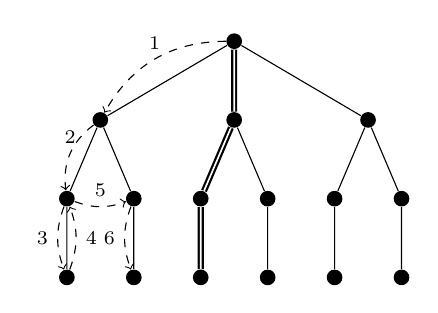
\begin{tikzpicture}[
    state/.style={circle, fill=black, inner sep=2pt},
    level distance=1.0cm,
    level/.style={sibling distance=17mm/#1}
]
\node [state] (a) {}
    child {node [state](b) {}
        child {node [state](c) {}
            child {node [state](d) {}}
            }
            child {node [state] (e) {}
            child {node [state] (f) {}}
            }
    }
    child {node [state](b1) {}
        child {node [state](b2) {}
            %child {node [state] {}}
            child {node [state](b3) {}}
            }
            child {node [state] {}
            child {node [state] {}}
            }
    }
    child {node [state] {}
        child {node [state] {}
            child {node [state] {}}
            }
            child {node [state] {}
            child {node [state] {}}
            }
    };
    \draw[->, dashed] (a) to [bend right=30] node [midway, above] {\scriptsize $1$} (b);
    \draw[->, dashed] (b) to [bend right=30] node [midway, above] {\scriptsize $2$} (c);
    \draw[->, dashed] (c) to [bend right=20] node [midway, left] {\scriptsize $3$} (d);
    \draw[->, dashed] (d) to [bend left=-20] node [midway, right] {\scriptsize $4$} (c);
    \draw[->, dashed] (c) to [bend right=20] node [midway, above] {\scriptsize $5$} (e);
    \draw[->, dashed] (e) to [bend right=20] node [midway, left] {\scriptsize $6$} (f);

    \draw[thick, double] (a) -- (b1);
    \draw[thick, double] (b1) -- (b2);
    \draw[thick, double] (b2) -- (b3);
\end{tikzpicture}%
\caption{\scriptsize Enumeration tree of the Lindner-Peikert algorithm for $3$-dimensional lattice with $\dvec = (3, 2, 1)$. }
\label{fig:TwoTreesLP}
\end{subfigure}
\hspace{10pt}
\begin{subfigure}[t]{0.47\textwidth}
\centering
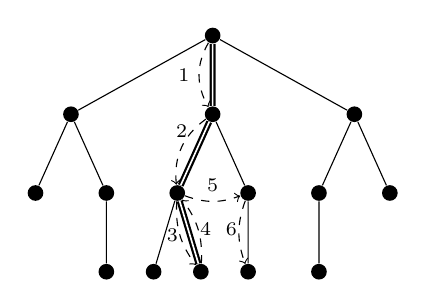
\begin{tikzpicture}[
    state/.style={circle, fill=black, inner sep=2pt},
    level distance=1.0cm,
    level/.style={sibling distance=18mm/#1}
]
\node [state] (a) {}
    child {node [state](b) {}
    	child {node [state] {} }
        child {node [state](c) {}
            child {node [state](d) {}}
            }
    }
    child {node [state](b1) {}
        child {node [state](b2) {}
            child {node [state] {}}
            child {node [state](b3) {}}
            }
            child {node [state](j) {}
            child {node [state](h) {}}
            }
    }
    child {node [state] {}
        child {node [state] {}
            child {node [state] {}}
            }
        child {node [state] {}}
    };
    \draw[->, dashed] (a) to [bend right=30] node [midway, left] {\scriptsize $1$} (b1);
    \draw[->, dashed] (b1) to [bend right=30] node [midway, above] {\scriptsize $2$} (b2);
    \draw[->, dashed] (b2) to [bend right=20] node [left, xshift=1mm] {\scriptsize $3$} (b3);
    \draw[->, dashed] (b3) to [bend left=-20] node [right, xshift=-1mm] {\scriptsize $4$} (b2);
    \draw[->, dashed] (b2) to [bend right=20] node [midway, above] {\scriptsize $5$} (j);
    \draw[->, dashed] (j) to [bend right=20] node [left, yshift=.4mm, xshift=1mm] {\scriptsize $6$} (h);

    \draw[thick, double] (a) -- (b1);
    \draw[thick, double] (b1) -- (b2);
    \draw[thick, double] (b2) -- (b3);
\end{tikzpicture}
\caption{\scriptsize Enumeration tree of the Generalized Pruning algorithm realized via some bounding function $\B$. As opposed to the left figure, the number of children varies for nodes on the same level.}
\label{fig:TwoTreesPrun}
\end{subfigure}
    \caption[Enumeration trees]{\footnotesize Enumeration tree of the Lindner-Peikert Algorithm (left) and the Generalized Pruning (right). The roots correspond to the initial call, the leaves contain the candidate error-vectors and the corresponding lattice vectors. The double-line represents the path (i.e.\ the choices of hyperplanes) that would have been chosen by the Babai's $\NP$ Alg.~\ref{alg:Babai}. The dashed curved arrows show the order of tree-traversals. On the left, the left-most child is visited first (usual depth-first tree-traversal). On the right, the `best' (w.r.t.\ the error-length)  child is chosen first (the \emph{best-first} traversal). 
    }
\label{fig:EnumTrees}
\end{figure}

\paragraph{Spherical and Linear-Length Pruning.} 

Note that the error-vector $\evec' = \sum_i e_i' \frac{\wbvec_i}{ \| \wbvec_i \|}$ is not explicitly bounded during the Lindner-Peikert's enumeration. 
It is done implicitly via restricting its individual coordinates $e_i'$. Each coordinate $e_i'$ is obtained by going one level down the enumeration tree: on level $k$ we compute $\evec'^{(k)} = \sum_{i=k+1}^m e_i' \frac{\wbvec_i}{ \| \wbvec_i \|}$ by adding $e'_{k+1}\frac{\wbvec_i}{ \| \wbvec_i \|}$ to $\evec'^{(k+1)}$ for an appropriately chosen coordinate $e'_{k+1}$ (see line \ref{algline:LPComputeError} in Alg.~\ref{alg:LP}).
By the end of the enumeration, $\evec'^{(k)}$ builds a final output $\evec'$ and hence, this final $\evec'$ will have length greater than $\| \evec'^{(k)} \|$. 
A moment's thought reveals that it is reasonable to make the number of children for a node dependent on the length of the error $\| \evec'^{(k)} \|$ associated to this node: the smaller this length is, the more children we want this node to have as it is more likely to lead to the correct solution, while if $\| \evec'^{(k)} \| \gg \sqrt{m} \alpha q$ (i.e.\ the accumulated error-length exceeds the expected length of the \LWE error), we might as well choose no children at all and stop the recursion for this node. This is why we use the term `pruning' as we prune the enumeration tree at some unpromising nodes.

For example, the \emph{Spherical Pruning} (\cite{SchE94}) chooses the number of the children for a $k\th$-level node with $\|\evec'^{(k)} \|^2 = \sum_{i=k+1}^m e_i'^2$ as $\TLandau  \left( \frac{1}{\| \wbvec_k \|^2} ( m (\alpha q)^2 - \sum_{i=k+1}^m e_i'^2) \right)$. This choice exactly captures our intuition: the shorter the accumulated error, the more children a node is allowed to have. We divide by $ \| \wbvec_k \|^2$ to get the actual number of the hyperplanes we recurse on (i.e.\ the number of children). It is easy to see that a pruning strategy enumerates all possible error-vectors that lie within the ball $\Ball(\tvec, \alpha q)$. 

Another pruning strategy, the \emph{Linear-Length Pruning} (\cite{EC:GamNguReg10}), reduces the search space of the Spherical Pruning by allowing a $k\th$-level error-vector to have norm $\| \evec'^{(k)} \|^2 \leq \TLandau( (m-k+1) (\alpha q)^2)$. This upper bound is the expected length of an $(m-k+1)$-dimensional vector with Gaussian entries of width $\alpha q$. It results, as in case of the Spherical Pruning, in the output error-vectors having norm $\TLandau(m \sqrt{\alpha q})$, but it is more restrictive on the intermediate levels.

There are several other pruning strategies considered in \cite{EC:GamNguReg10}, all aiming at reducing the search space by pruning the enumeration tree more aggressively, thus reducing the running time but sacrificing success probability (and hence, they are called \emph{Extreme Pruning} with the most `extreme' case being Babai's $\NP$). 
\vspace{10pt} %
\paragraph{Generalized Pruning.} All the enumeration strategies considered here can be described via a family of bounding functions $\B^{(k)}: \Q_{\geq 0}^{m-k} \rightarrow \Q_{\geq 0}$, $1 \leq k \leq m$. In general, this function may not even be efficiently computable in practice. For example, Aono in \cite{Ao14} suggests a way to find an optimal $\B^{(k)}$ given the Gram-Schmidt basis $\wBMat$ via solving an $m$-dimensional optimization problem. But for our $\GenPrun$ algorithm (Alg.~\ref{alg:GenPrun}) and its analysis we assume an efficiently computable family $\B^{(k)}$ which is given as an additional input.

%
% Generalized Pruning
%
\begin{algorithm}[t]
\caption{Generalized Pruning Algorithm $\GenPrun(\BMat, \protect \xvec, \protect \tvec, \protect \evec', \B^{(k)})$}
\label{alg:GenPrun}
\textbf{Input:} $\BMat=(\bvec_1, \ldots, \bvec_m) \in \Z^{m \times m}, \xvec\in\Q^m, \tvec \in \xvec+\Span(\BMat), \evec'\in\Q^m, \B^{(k)}$ \hfill ($\evec'=\xvec=0$ in the initial call)\\
\textbf{Output:} A set of pairs $(\vvec,\evec')$ with $\vvec\in \xvec+\Lat(\BMat)$ and $\evec' = \tvec-\vvec$ corresponding error vector
%\vspace{8pt}
\begin{algorithmic}[1]
\State $\xvec^{(k)}\gets \xvec, \tvec^{(k)}\gets \tvec,\evec'^{(k)}\gets\evec'$ 
\State Let $\wBMat\gets\GSO(\BMat)$
\If {$k=0$} \Return $\{(\xvec,\evec')\}$ \EndIf
\State Compute $c^{(k)}_1 \gets \bigScProd{\tvec^{(k)}}{\frac{\wbvec_k}{ \vphantom{\scalebox{1.6}x^2} \|\wbvec_k \|^2  }}$
\State
Let $e'_i = \ScProd{\evec'^{(k)}}{\frac{\wbvec_i}{\vphantom{\scalebox{1.6}x^2} \|\wbvec_i\|}}$ for $k< i \le m$ \Comment Coefficients of $\evec'$
\State Let $\Dmax^2 = \B^{(k)}(e'^2_m,\ldots,e'^2_{k+1})$ \Comment bound on distance of next hyperplanes \label{algline:GenPrunDmax}
\State Compute $c^{(k)}_j = \bigScProd{\xvec^{(k)}}{\frac{\wbvec_k}{\|{\wbvec_k}\|^2}} + i^{(k)}_j$ for all $i^{(k)}_j \in \Z$ s.t.\
$\abs{c_1^{(k)} - c_j^{(k)}}^2 \cdot \|\wbvec_k \|^2 \leq \Dmax^2$ \label{algline:GenPrunChoosePlane}
\For {\textbf{each} $(i^{(k)}_j, c^{(k)}_j)$} 
		\State $\xvec^{(k-1)}_j \gets \xvec^{(k)}+i^{(k)}_j \bvec_k$ \label{algline:GenPrunChooseTranslate}
		\Comment $U_j^{(k-1)} = \xvec^{(k-1)}_j+\Lat(\BMat^{(k-1)})$ are the nearby planes
		\State $\evec'^{(k-1)}_j \gets \evec'^{(k)} + (c^{(k)}_1-c^{(k)}_j)\wbvec_k$
		\State $\tvec^{(k-1)}_j =\tvec^{(k)} - (c^{(k)}_1-c^{(k)}_j)\wbvec_k$ \Comment Project onto $U_j^{(k-1)}$ 
\State \Return $\bigcup_j \GenPrun ((\bvec_1,\ldots,\bvec_{k-1}), \xvec^{(k-1)}_j,\tvec^{(k-1)}_j,\evec'^{(k-1)}_j, \B^{(k)})$
\EndFor
\end{algorithmic} 
\end{algorithm}

The algorithm computes the maximal allowed distance (denoted $\Dmax$) to the next hyperplanes (line \ref{algline:GenPrunDmax} of Alg.~\ref{alg:GenPrun}) and chooses only the hyperplanes for which $e'^2_k$ satisfies $e'^2_k < \B^{(k)} (e'^2_m, \ldots, e'^2_{k+1}) = \Dmax^2$. The search region of \GenPrun is
\begin{equation*} 
	V_{\GP} = \Bigl\{ \evec' = \sum_k e'_k \frac{\wbvec_k }{\| \wbvec_k \| } \colon e_k^2 \leq \B^{(k)}(e'^2_m, \ldots, e'^2_{k+1}) \; \forall k \Bigr\}.	
\end{equation*}

The algorithm successfully solves the \LWE problem if the \LWE error-vector $\evec$ is contained in the search region $V_{\GP}$. It is easy to see that Generalized Pruning captures all the enumeration strategies discussed here. Namely,

\begin{itemize}
	\item $\B^{(k)}(e'^2_m, \ldots, e'^2_{k+1}) = \left( \frac{\| \wbvec_k \|}{2} \right)^2 $: Babai's $\NP$
	\item $\B^{(k)}(e'^2_m, \ldots, e'^2_{k+1}) = \left( \frac{d_k \| \wbvec_k \|}{2} \right)^2 $: Lindner-Peikert's $\NPs$
	\item $\B^{(k)}(e'^2_m, \ldots, e'^2_{k+1}) = \TLandau(m (\alpha q)^2) - \sum_{i=k+1}^m e'^2_i$: Spherical Pruning
	\item $\B^{(k)}(e'^2_m, \ldots, e'^2_{k+1}) = \TLandau( (m-k)(\alpha q)^2) - \sum_{i=k+1}^m e'^2_i $: Linear Pruning
	\item $\B^{(k)}(e'^2_m, \ldots, e'^2_{k+1}) = R_k^2 -  \sum_{i=k+1}^m e'^2_i$: pruned strategy with some level-dependent bounds $R_k$.  
\end{itemize}
 
All the extreme pruning approaches of \cite{EC:GamNguReg10} as well any numerically optimized strategy are covered by the last choice of $\B^{(k)}$.

For the analysis, we extend $\B^{(k)}$ to real-valued arguments so that we can apply the algorithm to a continuous Gaussian.

\paragraph{Analysis.} As before, we are interested in the ratio $\rho(\GP) = \frac{T(\GP)}{\Psucc(\GP)}$ ($\GP$ is used as a shorthand for Generalized Pruning). A family of bounding functions $\B^{(k)}$ defines the search region on level $k$ as
\begin{equation}\label{eq:VGP}
	V_{\GP}(k) =  \Bigl\{ \evec' = \sum_{i=k+1}^m e'_i \frac{\wbvec_i }{\| \wbvec_i \| } \colon e_j^2 \leq \B^{(j)}(e'^2_m, \ldots, e'^2_{j+1}) \;  k < j \leq m \Bigr\}.
\end{equation}

Let $N_k$ be the number of nodes at level $k$ and $p_k$ be the probability that the correct solution is retained on level $k$ (i.e.\ there exists a node with $\evec^{(k)}$ that can be extended to the correct \LWE error $\evec$ by traversing the tree down to the last level). We define a \emph{reasonable pruning} via requiring a set of conditions to be met by $\B^{(k)}, N_k,  p_k$. We assume that the error we seek for, follows a continuous Gaussian with parameter $\alpha q$ and that $ \| \wbvec_m \| < \alpha q < \| \wbvec_1 \| $. The latter is satisfied by the choice of $\beta$.

\begin{definition}[Reasonable Pruning] \label{def:ReasonablePruning}
Let $k^*$ be the maximal level s.t.\ $\| \wbvec_{k^*} \| > \alpha q$. The Generalized Pruning algorithm with the associated $\B^{(k)}$ is \emph{reasonable} if the following conditions are satisfied
 \begin{enumerate}
 	\setlength\itemsep{0.1em}
 	\item $\B^{(k)}(e'^2_m, \ldots, e'^2_{k+1}) + \sum_{i=k+1}^m e'^2_i = \TLandau(m (\alpha q)^2)$ 
 	\item $\Psucc(\GP) \geq 2^{-\bigO(m)} \cdot p_{k^*}$
 	\item $N_k \leq 2^{\bigO(m)} \cdot N_{k^*}$ for $k \leq k^*$
 	\item $\frac{N_{k-1}}{N_k} = \WLandau(1)$ for $k \geq k^*$
 	\item $V_{\GP}(k^*)$ is convex.
 \end{enumerate}
\end{definition} 

Informally, the conditions in Def.~\ref{def:ReasonablePruning} have the following meaning: Condition 1 implies that we prune the nodes with the accumulated error larger than the expected length of the \LWE error. Conditions 2 and 3 mean that as soon as the correct error survived until the `critical' level $k^*$, we can find $\evec$ with high probability (Condition 2) at essentially no additional cost (Condition 3). For example, from $k^*$ down, we can start the Babai's $\NP$ algorithm. Condition 4 ensures that for levels above $k^*$ we choose \emph{at least} a constant number of hyperplanes (line \ref{algline:GenPrunChoosePlane} in Alg.~\ref{alg:GenPrun}) to recurse on. Note that on these upper levels we have $\| \wbvec_k \| < \alpha q$ for $k>k^*$, so we must have $\WLandau(1)$ hyperplanes at distance at most $\alpha q$.

We elaborate on the convexity condition a bit more. Let us take a closer look at the search region $V_{\GP}$. From the way the error-vectors $\evec'^{(k)}$ are constructed during the algorithm, the number of nodes at level $k$, denoted $N_k$, is the number of points in $V_{\GP}(k) - \evec$ that belong to the lattice $\Lat(\wbvec_m, \ldots, \wbvec_{k+1})$, i.e.\ to the orthogonal projection of $\Lat(\BMat)$ onto $\Span(\bvec_1, \ldots, \bvec_k)$ (the shift by $\evec$ does not change $N_k$ asymptotically but is needed for the proof below). The Gaussian Heuristic suggests that
\begin{equation*} %\label{eq:GaussHeuristic}
	N_k \approx \frac{\vol V_{\GP}(k)}{\prod_{i=k+1}^m \| \wbvec_i \|}.
\end{equation*}

We could use this approximation in our theorem below, but since it is enough in our setting to upper-bound $N_k$ up to a factor of $2^{\bigO(m)}$, we can prove the above equation by relying on a variant of Minkowski's Convex Body Theorem. 
Roughly, this theorem tells us that if an $m$-dimensional 0-symmetric convex point-set ($V_{\GP}(k)$ for us) has volume larger than the volume of a lattice, then it contains a non-zero point of this lattice. 

The generalization of this result is due to Rado \cite{R46}: instead of a 0-symmetric convex set, he considers a non-negative integrable function $f(\xvec)$  and connects the quantity $\sum_{\vvec \in \Lat} f(\vvec)$ with the value $\mathcal{V}(f) =~ \int_{- \infty < x_i < \infty} f(\xvec) \d \xvec$. The convexity condition of the set is replaced by the quasi-concavity condition for $f$: for a linear map ${\Lambda}$ from an $m$-dimensional vector space into itself, the function $f$ must satisfy $f(\Lambda \xvec - \Lambda \yvec) \geq \min \{ f(\xvec), f(\yvec) \}$.
Later in Thm.~\ref{thm:GenPrunRunTime}, we consider $\Lambda$ acting like $\Lambda \xvec = \tfrac{1}{2} \xvec$. 
Minkowski's Convex Body Theorem is a special case of the Thm.~\ref{thm:Rado} for $f(\xvec)$ being a characteristic function of a convex symmetric set $V$ in which case $\mathcal{V}(f) = \vol V$.

\begin{thm}[Rado's generalization of Minkowski's Convex Body Theorem] \label{thm:Rado}
Let $f(\xvec)$ be a non-negative integrable function with the property $f(\Lambda \xvec - \Lambda \yvec) \geq \min \{ f(\xvec), f(\yvec) \}$ for all $\xvec, \yvec \in \R^m$ and a linear map $\Lambda: \R^m \rightarrow \R^m$. Then
\begin{equation} \label{eq:RadosThm}
	f(\zerovec) + \tfrac{1}{2} \sum_{\zerovec \neq \vvec \in \Lat} f(\vvec) \geq \frac{\abs{\det \Lambda}}{\det (\Lat)} \mathcal{V}(f),
\end{equation}
for every lattice $\Lat$, where 
\[
\mathcal{V}(f) = \int\limits_{\substack{ - \infty < x_i < \infty \\ 1 \leq i \leq m }} f(\xvec) \d \xvec,
\] 
and $\det(\Lambda)$ is the determinant of the $m \times m$ matrix that defines the transformation $\Lambda$.
\end{thm}
Following the proof of the theorem (see the book of Cassels \cite[Chap.\ III]{Cas97} for a comprehensive proof) and setting $\Lambda \xvec = \tfrac{1}{2} \xvec$ (so $\abs{\det \Lambda} = 2^{-m}$), we observe that up to $2^{\bigO(m)}$ the inequality given in Eq.~\eqref{eq:RadosThm} is an equality, so in our proof we rely on the fact that
\begin{equation} \label{eq:RadoEq}
f(\zerovec) + \tfrac{1}{2} \sum_{\zerovec \neq \vvec \in \Lat} f(\vvec) = \frac{2^{\pm \bigO(m)}}{\det (\Lat)} \mathcal{V}(f).
\end{equation}

Now we have the tools to present the main theorem of this section \emph{without} relying on the Gaussian Heuristic. 
We apply Eq.~(\ref{eq:RadoEq}) to the function $f(\xvec) = \tfrac{1}{(\alpha q)^{k^*}} \int_{V_{\GP}(k^*)} \exp \left( \frac{-\pi \| \yvec \|^2}{(\alpha q)^2} \right) \d \yvec$ and to the lattice $\Lat(\wbvec_m, \ldots, \wbvec_{k^*+1})$, where $k^*$ is the `critical' level as in Def.~\ref{def:ReasonablePruning}. $f(\xvec)$ is the convolution of the Gaussian density function with the characteristic function of our convex search region $V_{\GP}(k^*)$ and hence, it satisfies the quasiconcavity condition of Thm.~\ref{thm:Rado}. 

\begin{thm}[Analysis of the $\GenPrun$ Algorithm~\ref{alg:GenPrun}] \label{thm:GenPrunRunTime}
Given a $\beta = \TLandau(n)$-\BKZ reduced basis that arises from $m = \TLandau(n)$ \LWE-samples with parameters $(n, q=\bigO(n^{\cq}), \alpha = \bigO(1 / n^{\ca}) )$ for positive constants $\cq >\ca$ s.t.\ $\frac{m}{2 \beta} + \frac{n}{m} \cq - \ca >0$, any reasonable (as in Def.~\ref{def:ReasonablePruning}) pruning algorithm $\GP$ has an expected (over the choice of $\evec$) running time/success probability trade-off
\[
	\rho(\GP) = \frac{\E[T(\GP)]}{\Psucc(\GP)} = 2^{\frac{1}{2} \bigl(\frac{m}{2\beta}-\ca + \frac{n}{m} \cq  \bigr)^2 (1+\smallo(1)) \cdot \beta\log\beta},
\]
with $\poly(m)$ memory (using depth-first search) assuming the Geometric Series Assumption holds and the \LWE error follows a continuous Gaussian distribution.
\end{thm}

\begin{proof}
	The amount of work done on one node of the enumeration tree of Alg.~\ref{alg:GenPrun} is clearly $\poly(m)$, so the total running time is $T(\GP) = \poly(m) \cdot \sum N_k$. For the `critical' level $k^*$ (i.e.\ maximal level with $\| \wbvec_{k^*} \| > \alpha q$), we have $N_i < 2^{\bigO(m)}$ for all $i$ (for $i<k^*$ due to Condition 3 in Def.~\ref{def:ReasonablePruning}, for $i>k^*$ by the definition of $N_k$). So for a reasonable pruning strategy, it holds that
	\[
		T(\GP) = 2^{\bigO(m)} N_{k^*}.
	\]
	As discussed above, $N_{k^*}$ is (up to $2^{\bigO(m)}$) the number of lattice vectors $\vvec \in \Lat (\wbvec_m, \ldots, \wbvec_{k^* +1})$ that lie in the convex region $V_{\GP} - \evec$. Taking the expectation over the choice of $\evec$, 
	\[
		\E_{\evec}[N_{k^*}] = \sum_{\vvec \in \Lat (\wbvec_m, \ldots, \wbvec_{k^* +1})} f(x) \qquad \text{where} \qquad f(\xvec) = \tfrac{1}{(\alpha q)^{k^*}} \int\limits_{V_{\GP}(k^*)} \exp \left( \frac{-\pi \| \yvec \|^2}{(\alpha q)^2} \right) \d \yvec.
	\]
	This expectation is essentially the left-hand side of Eq.~(\ref{eq:RadoEq}). Note that $f(x)$ is quasiconcave (as it is a convolution of two log-concave functions: the Gaussian density function and the characteristic function of the convex region $V_{\GP}$). For $\Lat = \Lat(\wbvec_m, \ldots, \wbvec_{k^* +1})$, we obtain
	\begin{align*}
			\E_{\evec}[N_{k^*}] &= \frac{2^{\pm \bigO(m)}}{\det (\Lat)} \int f(\xvec) \d \xvec = 
			\frac{2^{\pm \bigO(m)}}{\det (\Lat)} \int\limits_{V_{\GP}(k^*)} \int\limits_{\substack{ - \infty < y_i < \infty \\ 1 \leq i \leq m }} \frac{1}{(\alpha q)^{k^*}} \exp \left( \frac{-\pi \| \yvec \|^2}{(\alpha q)^2} \right) \d \yvec \d \xvec =  \\
			&= \frac{2^{\pm \bigO(m)} \vol V_{\GP}(k^*)}{\det (\Lat)}.  
	\end{align*}
	If the pruning is reasonable, we have $\Psucc(\GP) = 2^{-\bigO(m)} \cdot p_{k^*}$, where $p_{k^*}$ is the probability that there exist a vector in $V_{k^*}$ s.t.\ its $m-k^*$ coordinates extend to the \LWE error-vector, yielding
	\begin{align*}
		\frac{\E[T(\GP)]}{\Psucc(\GP)} &= \frac{2^{\pm \bigO(m)} \vol V_{\GP}(k^*)}{\det (\Lat) \cdot \tfrac{1}{(\alpha q)^{m-k^*}} \int\limits_{\xvec \in V_{\GP}(k^*)} \exp(- \tfrac{\pi \| \xvec \|^2}{(\alpha q)^2}) \d \xvec} = 
		\frac{2^{\pm \bigO(m)} \cdot (\alpha q)^{m-k^*} \vol V_{\GP}(k^*) }{\prod_{i=m-k^*}^m \| \wbvec_i \| \cdot \int\limits_{\xvec \in V_{\GP}(k^*)} \exp(- \tfrac{\pi \| \xvec \|^2}{(\alpha q)^2})} = \\
		&= \frac{2^{\pm \bigO(m)} \cdot (\alpha q)^{m-k^*} \int_{\xvec \in V_{\GP}(k^*)} 1 \d \xvec}{\prod_{i=m-k^*}^m \| \wbvec_i \| \cdot \int_{\xvec \in V_{\GP}(k^*)} 1 \d \xvec} = 
		2^{\frac{1}{2} \bigl(\frac{m}{2\beta}-\ca + \frac{n}{m} \cq  \bigr)^2 (1+\smallo(1)) \cdot \beta\log\beta},
	\end{align*} 
	where for the third equality we used Condition 1 in Def.~\ref{def:ReasonablePruning} stating that $e^{-\bigO(m)} \leq \exp(- \tfrac{\pi \| \xvec \|^2}{(\alpha q)^2}) \leq 1$ for any $\xvec \in V_{\GP}(k^*)$.
\end{proof}

We remark that for a pruning strategy that has $\Psucc \leq p_{k^*}$ and $T \geq \poly(m) N_{k^*}$, the result of Thm.~\ref{thm:GenPrunRunTime} gives a lower bound on the trade-off $\rho$ for such a strategy. 

Finally, note that the Lindner-Peikert $\NPs$ algorithm is a corner-case of a reasonable pruning: in the corners of the parallelepiped-shaped search region $V_{\NPs}$ Condition 1 is not satisfied. This is why we analyzed it separately. Now we can move on to the discussion on the total complexity of the \BDD attack on \LWE where we balance the running time of the reduction and enumeration phases.

\subsection{Total complexity of \LWE decoding} \label{sec:Balance}

The \BDD attack on \LWE is a two-phase algorithm: the enumeration (phase 2) in performed on a $\beta$-\BKZ reduced basis (phase 1). So far we have been discussing the second phase -- enumeration -- ignoring the complexity of the reduction. By now we have the quantity $\rho(\ENUM) = \frac{T(\ENUM)}{\Psucc(\ENUM)}$, and we can finally turn our attention to the total complexity of the attack taking into account the reduction: $\rho(\BDD) = \frac{T(\BKZ)+T(\ENUM)}{\Psucc(\ENUM)}$.

$T(\BKZ)$ is determined by the input parameter $\beta$ or, more precisely, by the running time of an \SVP-solver on a lattice of dimension $\beta$ (the dimension of the original lattice -- $m$ for \LWE -- only affects a polynomial factor in $T(\BKZ)$). We have already mentioned two ways to instantiate an \SVP-solver in Chap.~\ref{sec:PrelimLattices}:
	\begin{itemize}
		\item[--] $T(\BKZ) = 2^{\cBKZ \cdot \beta \log \beta + \smallo(\beta \log \beta) }$ with $\poly(\beta)$ space complexity due to Kannan \cite{STOC:Kannan83} for $\cBKZ = \TLandau(1)$ (Hanrot and Stehl\'{e} in \cite{C:HanSte07} estimate $\cBKZ = \tfrac{1}{2e}$),
		\item[--] $T(\BKZ) = 2^{\cBKZ \cdot \beta  + \smallo(\beta)}$ with $2^{\bigO(\beta)}$ memory due to Micciancio-Voulgaris \cite{STOC:MicVou10} and Aggarwal et al.\ \cite{STOC:ADRS15} (for the former, $\cBKZ = 2$, and for the latter $\cBKZ = 1$; the space complexity is $2^{\beta + \smallo(\beta)}$ for both algorithms).
	\end{itemize}  
	
From now on, we ignore the $\smallo(\cdot)$-terms in the exponents. The above two cases result into two statements for the complexity of the \BDD attack. We start with Kannan's \SVP. We make a distinction between enumerations that achieve a constant success probability (Lindner-Peikert $\NPs$, Spherical or Linear-Length Pruning) and those that have an arbitrarily small success probability (Babai's $\NP$, Extreme Pruning).
As in the previous sections, we assume the \LWE error follows a continuous Gaussian distribution with parameter $\alpha q$.
\begin{thm}[Super-exponential \BDD-attack on \LWE] \label{thm:BalanceSuperExp}
	The \LWE problem with parameters $(n, q=\bigO(n^{\cq})$, $\alpha = \bigO(1 / n^{\ca}) )$ where $\cq, \ca = \TLandau(1)$, can be solved via \BDD with (1) a $\beta=\TLandau(n)$-basis reduction running in time $2^{\cBKZ \beta \log \beta}$ and (2) any enumeration algorithm $\ENUM \in \{ \GenPrun, \NPs \}$ using the optimal choice of $m = \left( \frac{2 \cq}{\sqrt{2 \cBKZ}+\ca} + \smallo(1) \right) \cdot n$ samples in time 
\begin{align*}
		T(\BDD) = 2^{ \left( \cBKZ \cdot \frac{2 \cq}{(\sqrt{2 \cBKZ}+\ca)^2} \right) \cdot n \log n},
\end{align*}
	if $\Psucc(\ENUM) = 1 - \smallo(1)$. For arbitrary $\Psucc(\ENUM)$, the above quantity is a lower bound for $\rho(\BDD)$.
\end{thm}

\begin{proof}
	Assume we run an enumeration algorithm with $\Psucc(\ENUM) = 1 - \smallo(1)$. Investing more time in the reduction (i.e.\ improving the quality of the output basis) results in a faster enumeration, so the total running time $T(\BDD) = T(\BKZ)+ T(\ENUM)$ is minimized if the two phases are balanced. Thms.~\ref{thm:LPRunTime} resp.\ \ref{thm:GenPrunRunTime} give $T(\NPs)$ resp.\ $T(\GenPrun)$. On the logarithmic scale, the balancing condition $T(\BKZ) = T(\ENUM)$ is equivalent to (omitting the $\smallo(1)$-terms)
	\[
		\frac{1}{2} \left( \frac{m}{2 \beta} + \frac{n}{m} \cq - \ca \right)^2 \beta \log \beta = \cBKZ \beta \log \beta.
	\]
	This equation yields $\beta = \frac{1}{2} \frac{m}{\sqrt{2 \cBKZ}-(n/m)\cq + \ca}$. This expression attains its minimum at $m = \frac{2 \cq}{\sqrt{2 \cBKZ} + \ca}$, from where the first theorem statement easily follows. Note that for a constant success probability of enumeration, $\rho(\BDD) = \TLandau(T(\BDD))$.
	
	For arbitrary $\Psucc(\ENUM)$, we have $\rho(\BDD) = \frac{T(\BKZ)}{\Psucc(\ENUM)}+\rho(\ENUM) \geq T(\BKZ) + \rho(\ENUM)$, and we have just computed $T(\BKZ) + \rho(\ENUM)$. 
\end{proof}

Now we consider the case when a lattice-basis reduction has a \emph{single} exponential complexity $2^{\cBKZ \cdot \beta}$. Recall Thm.~\ref{thm:GenPrunRunTime} shows that for $\ENUM =  \GenPrun$, $\rho(\ENUM) = 2^{\TLandau(\beta \log \beta)}$. Cor.~\ref{cor:BabaiAndLP} states the same trade-off for the Babai's $\NP$ and Lindner-Piekert $\NPs$ algorithms.

So asymptotically, it is optimal to reduce the input basis to a point where the cost of enumeration switches from super-exponential to polynomial since in this case, $T(\BDD)$ is dominated by the reduction and stays singe-exponential. In the next theorem, we find a value of $\beta$ for which the reduction phase will produce a basis required for a $\poly(m)$-time enumeration that will produce the correct output with success probability almost 1. This enumeration may be either the Babai's $\NP$, Lindner-Peikert $\NPs$ or any (reasonable) pruning strategy with $\poly(m)$ number of nodes. 

\begin{thm}[Single-exponential \BDD-attack on \LWE] \label{thm:BalanceSingleExp}
	The \LWE problem with parameters ($n$,\linebreak $q=\bigO(n^{\cq})$, $\alpha = \bigO(1 / n^{\ca}) $) where $\cq, \ca = \TLandau(1)$ can be solved via \BDD with (1) a $\beta= \Bigl( \frac{2 \cq}{\ca^2} + \smallo(1) \Bigr) \cdot n$-basis reduction running in single-exponential time $2^{\cBKZ \beta}$ and (2) $poly(m)$-time enumeration algorithm using the optimal choice $m = \left( \frac{2 \cq}{\ca} + \smallo(1) \right) \cdot n$ of samples in time
	\[
		T(\BDD) = 2^{ \Bigl(\cBKZ \cdot \frac{2 \cq}{\ca^2} + \smallo(1) \Bigr) \cdot n}
	\]
	with $\Psucc(\BDD) = 1 - \smallo(1)$.
\end{thm}

\begin{proof}
 To guarantee a constant success probability and polynomial running time for enumeration, we need to ensure that the last Gram-Schmidt vector of the basis returned by $\beta$-reduction satisfies $\|  \wbvec_m\| > \alpha q$. This is equivalent to (cf.\ Cor.~\ref{cor:BabaiAndLP}) $\frac{m}{2 \beta} - \ca + \frac{n}{m}\cq  < 0$, so $\beta$ must be set as
 \[
 	\beta > \frac{1}{2} \frac{m}{\ca - \cq \cdot n/m}. 
 \]
 
 This value is minimized for $m = \frac{2 \cq}{\ca}$ yielding $\beta > \frac{2 \cq}{\ca^2} \cdot n$. The theorem statement follows directly from plugging this value in the running time of the reduction. 
\end{proof}

This theorem concludes the discussion on the two-phase \BDD attack on \LWE. In the following section, we briefly discuss some other lattice-based methods to solve \LWE.

\subsection{Other lattice-based algorithms for \LWE} \label{sec:OtherAttacks}

To provide a complete picture on lattice-based attacks, we briefly describe two other algorithms one can use to solve \LWE. First is the so-called Kannan's homogenization technique \cite{Kan87}, which allows us to convert a $\CVP$ (resp.\ $\BDD$) instance to an $\SVP$ (resp.\ $\uSVP$) instance in a higher-dimensional lattice (the approximation parameter $\gamma$ in $\uSVP$ depends on the promise given in the original \BDD instance). This approach is know as the \emph{embedding} technique. We show the running time of this attack when applied to $\LWE$ in Thm.~\ref{thm:Embed}. An analogous result was presented in \cite{APS15} but our choice of $m$ is different.

The second approach we consider, the so-called \emph{dual} attack, tackles the \emph{decisional}-\LWE (see Def.~\ref{def:decLWE}) by solving $\appSVP$ (for an appropriate choice of $\gamma$) in the lattice dual to the \LWE lattice. 

\paragraph{Embedding.} $\mkern-6mu$ Assume a \CVP instance $(\Lat(\BMat), \tvec)$ has a solution $\vvec \in \Lat(\BMat)$. Consider a higher-dimensional lattice $\LEmb (\BMat, \tvec)$ generated by the columns of the matrix
\begin{equation} \label{eq:BEmbed}
	\BMat' = \begin{pmatrix}
				\BMat & \tvec \\
				0 & \tau
			\end{pmatrix},
\end{equation}
 where $\tau$, known as the \emph{embedding factor}, is chosen such that the shortest vector in $\LEmb(\BMat, \tvec)$ is of the form $(\vvec, e)$ for $e \neq 0$. In other words, solving $\SVP$ on $\LEmb(\BMat, \tvec)$ leads to a solution of the original $\CVP$ problem. Note that $\tau$ should not be too small (in the worst-case $\CVP$ instance, $\tau$ is $\tfrac{1}{2} \lambda_1(\Lat(\BMat))$), otherwise the last column of the matrix $\BMat'$ may be used too often and the returned shortest vector may be the closest to a multiple of $\tvec$. On the other hand, $\tau$ should not be too large, otherwise the returned shortest vector will lie in $\Span(\BMat)$ giving no information on the solution to \CVP. 
 
 The embedding technique becomes more powerful if we know some information on the $\CVP$ instance we are given. In the $\BDD$ problem, for instance, we have a promise that the target vector is much closer to the solution-vector $\vvec$ than to any other lattice-vector. In this case, Kannan's technique leads us to the $\uSVP$ problem. In case of \LWE, we know that $\| \tvec - \vvec \| = \| \evec \| = \TLandau(\alpha q \sqrt{m})$, and, further, we know $\lambda_1(\BMat)$. It allows us to estimate $\lambda_1$ and $\lambda_2$ in $\LEmb(\BMat, \tvec)$ as $\lambda_1^2= \| \evec \|^2 + \tau^2$, $\lambda_2 = \lambda_1(\BMat)$, and hence, we know the gap of the lattice $\LEmb$. This gives us a bound on parameter $\gamma = \frac{\lambda_2}{\lambda_1}$ in the $\uSVP$ problem we are solving. 

We solve the $\uSVP$ problem via lattice-basis reduction. From Eq.~(\ref{eq:b1norm}), we know that an $m$-dimensional $\beta$-\BKZ reduced lattice, gives a $\beta^{\frac{m}{2 \beta}}$ approximation to a shortest vector of the lattice. Hence, as soon as the first (the shortest) vector of the reduced basis satisfies $\| \bvec_1 \| < \lambda_2(\LEmb(\BMat, \tvec))$, this vector is the shortest in $\LEmb(\BMat, \tvec)$ and, consequently, is the solution to $\uSVP$. All that remains is to determine the \BKZ parameter $\beta$ for which the first vector meets the requirement. 

In the theorem below, we consider the two possible running times of $\BKZ$, super-exponential (resp.\ single-exponential) as $f(\beta) = \beta \log \beta + \smallo(\beta \log \beta)$ (resp.\ $f(\beta) = \beta + \smallo(\beta)$). We omit the $\smallo(\cdot)$-terms. The space complexity of the attack is polynomial in the first case and exponential in $\beta$ in the second.
\begin{thm}[Complexity of the Embedding Attack on \LWE] \label{thm:Embed}
	The \LWE problem with parameters $(n, q=\bigO(n^{\cq}), \alpha = \bigO(1 / n^{\ca}) )$ where $\cq, \ca = \TLandau(1)$, can be solved via \emph{embedding} using a $\beta$-\BKZ reduction with $T(\BKZ) = 2^{\cBKZ \cdot f(\beta)}$, where either $f(\beta) = \beta$, or $f(\beta) = \beta \log \beta$ using the optimal choice of $m = \left( \frac{2 \cq}{\ca} + \smallo(1) \right) \cdot n$ of \LWE samples in time
	\[
		T(\Embed) = 2^{\left( \cBKZ \cdot \frac{2\cq}{\ca^2} + \smallo(1) \right) f(n)}.
	\]
\end{thm}

\begin{proof}
	Let $\BMat$ be a matrix that arises from $m$ \LWE samples and let $\LEmb(B, \tvec)$ be the corresponding $m+1$-dimensional lattice generated by the matrix defined in Eq.~(\ref{eq:BEmbed}). Let us estimate the first two successive minima $\lambda_1$, $\lambda_2$ for the embedded lattice. Setting the embedding factor $\tau = \TLandau(\| \evec \|)$, we obtain
	\[
		\lambda_1^2(\LEmb(\BMat, \tvec)) = \| \evec \|^2 + \tau^2 = \TLandau((\alpha q)^2 m).
	\]
	For a $q$-ary \LWE lattice, we have $\lambda_1(\Lat(\BMat)) =\min \{ q, \sqrt{m} q^{1 - n/m} \}$. For our choice of $m$, Minkowski's bound is always smaller, leading to
	\[
		\lambda_2(\LEmb(\BMat, \tvec)) = \lambda_1(\Lat(\BMat)) \leq \sqrt{m} q^{1 - n/m}.
	\] 
	The value of $\beta$, for which the $\beta$-reduced basis achieves an approximation of $\frac{\lambda_2(\LEmb(\BMat, \tvec))} { \lambda_1(\LEmb(\BMat, \tvec))}$, is given by
	\[
		\beta^{m / (2 \beta)} = \frac{\lambda_2(\LEmb(\BMat, \tvec))}{\lambda_1(\LEmb(\BMat, \tvec))} = \TLandau \left( \frac{q^{1-n/m}}{\alpha q} \right),
	\]
	assuming Minkowski's bound holds with equality. This is equivalent to $\beta = \left( \frac{2 \cq}{\ca^2} + \smallo(1) \right) \cdot n$. The minimum value for $\beta$ is attained at $m = \left( \frac{2 \cq}{\ca} + \smallo(1) \right) \cdot n$. 
\end{proof}

There is no surprise that the complexity of the embedding attack is exactly the same as the complexity of the two-phase \BDD attack with the single-exponential reduction followed by a polynomial-time enumeration (cf.\ Thm.~\ref{thm:BalanceSingleExp}). Both methods are, in fact, equivalent: performing a Babai-type (i.e.\ polynomial) enumeration on a reduced basis can be interpreted as embedding the target into the reduced basis and then size-reducing it (i.e.\ running \LLL). After such a procedure, the first vector reveals the closest vector.

\paragraph{Dual attack \hspace*{-8pt}}, originally considered in \cite{MicReg09} and further discussed in \cite{C:KirFou15}, solves the \emph{decisional}-\LWE. 

Given an \LWE instance $(\AMat, \tvec = \AMat\transpose \svec + \evec \bmod q) \in \Z_q^{n \times m} \times \Z_q^m$, instead of working with the lattice $\qLat(\AMat\transpose)$ (i.e.\ the image of $\AMat\transpose$) as we did so far, we make use of another $q$-ary $m$-dimensional lattice -- the kernel of $\AMat$:
\begin{align} \label{eq:DualLattice}
	\qLATTp (\AMat) = \{ \xvec \in \Z^m \colon \AMat \xvec = \zerovec \bmod q \}.
\end{align}
This lattice is the scaled dual to $\qLat(\AMat\transpose)$ with determinant $\det \qLATTp (\AMat) = q^n$ (the duality follows from the fact that $\qLATTp (\AMat) = q (\Lat(\AMat\transpose))^*$). A basis for this lattice can be easily formed from a (non-zero) matrix $\XMat$ that satisfies $\AMat \XMat = 0 \mod q$.

Assume we have found a short non-zero vector $\vvec \in \qLATTp (\AMat)$. Computing $w = \langle\vvec,\tvec\rangle \bmod q = \vvec^t (\AMat\transpose \svec + \evec ) \mod q = \ScProd{\vvec}{\evec} \bmod q$, we can distinguish whether $\evec$ is uniform or Gaussian. 
If $\evec$ is uniform, $w$ is also uniform, while if $\evec$ is Gaussian, $w = \sum_i v_i e_i$ is Gaussian with parameter $\alpha q \cdot \| \vvec \|$ (again, we assume the \LWE error follows a continuous Gaussian distribution). 
In the second case, the statistical distance between $w \bmod q$ and a uniform random variable $\bmod \ q$ or, a \emph{bias} of a continuous Gaussian with parameter $\alpha q \cdot \| \vvec \|$, is $\delta = 2^{-\bigO(\alpha^2 \| \vvec \|^2)}$. 
(To see this, we take a Fourier transform over $\Z_q$ of the Gaussian density function with standard deviation $\alpha q \| \vvec \|$ and evaluate at $1/q$). 
There exists an efficient distinguisher that has the advantage $\delta$ in deciding whether $w$ is uniform or Gaussian. 
For instance, [\cite{EC:DucTraVau15}, Lemma 10] shows that for Gaussian $w$ with standard deviation $s$ over $\Z_q$, $\E[\cos \bigl( \tfrac{2 \pi w}{q}\bigr)] \geq \frac{q}{\pi} \sin \left( \tfrac{\pi}{q}\right) e^{-2 \pi^2 s^2/q^2} $ (cf.\ line \ref{algline:decLWEDistinguish} in Alg.~\ref{alg:Dual}), while for a uniform $w \in \Z_q$, $\E[\cos \bigl( \tfrac{2 \pi w}{q}\bigr)] = 0$.

%
% DUAL algorithm
%
\setlength{\intextsep}{\medskipamount}
\begin{algorithm}[t]
\caption{ Dual attack on decisional-\LWE $\DUAL (\AMat, \protect \tvec, \eps)$}
\label{alg:Dual}
\textbf{Input:} $\AMat \in \Z^{m \times k}, \tvec \in \Z^m$ where  either (1) $\tvec = \AMat\transpose \svec + \evec \bmod q$ or (2) $\tvec$ is uniform from $\Z_q^m$  \\
\textbf{Output:} ``Yes'' if $\tvec = \AMat\transpose \svec + \evec \bmod q$, ``No'' otherwise.
\begin{algorithmic}[1]
	\State Compute $\XMat$ s.t.\ $\AMat \XMat = 0 \bmod q$ via Gaussian elimination
	\State $\BMat \gets$ $\beta$-\BKZ ($\qLat(\XMat)$) with $\beta = \left( \frac{2 \cq}{(1/2 + \ca)^2} + \smallo(1) \right) \cdot n$\Comment{
	\scriptsize
	Although we do not know $\ca$, we can approximate it by  \hspace*{9.1cm} trying several $\ca \in [0, \cq]$ in a binary-search manner} 
	\normalsize
	\If {$ \exists \vvec \in \Lat(\BMat)$ s.t.\ $\|\vvec \| =  \bigO(n^{1/2+\ca - \eps})$} 
		\normalsize
		\If {$\cos \left( \frac{ 2 \pi \langle{\vvec},{\tvec} \mkern3mu\rangle} {q} \right)> \frac{q}{\pi} \sin \left( \frac{\pi}{q}\right) e^{-2 \pi^2  \cdot n^{1-\eps}}$} \label{algline:decLWEDistinguish}
			\State \Return ``Yes''
		\Else
			\State \Return ``No''
		\EndIf
	\EndIf
\end{algorithmic} 
\end{algorithm}

To keep the bias $\delta = 2^{-\bigO(\alpha^2 \| \vvec \|^2)}$ sub-exponential, we must have $\| \vvec \| = \bigO(n^{1/2+\ca - \eps})$ for any $\eps>0$. The following lemma estimates the value for $\beta$ s.t.\ a $\beta$-\BKZ reduction (now on $\qLATTp (\AMat)$) outputs $\vvec$ of desired length. 

\begin{lemma}[Decisional \LWE under the $\DUAL$ attack] \label{lem:DecisionalLWE}
The \emph{decisional}-\LWE problem with parameters $(n,$ $q=\bigO(n^{\cq})$, $\alpha = \bigO(1 / n^{\ca}) )$ where $\cq, \ca = \TLandau(1)$, can be solved via running a $\beta$-\BKZ reduction on the \emph{dual} lattice defined as in Eq.~(\ref{eq:DualLattice}) with $T(\BKZ) = 2^{\cBKZ \cdot f(\beta)}$, where either $f(\beta) = \beta$, or $f(\beta) = \beta \log \beta$, using the optimal choice of $m = \left( \frac{2 \cq}{1/2 + \ca} + \smallo(1) \right) \cdot n$ of samples in time
	\[
		T(\DUAL) = 2^{\left( \cBKZ \cdot \frac{2\cq}{(1/2+\ca)^2} + \smallo(1) \right) f(n)}.
	\]
with $\Psucc(\DUAL) = 2^{-\bigO(n^{1-\eps})}$ for $\eps>0$.
\end{lemma}

\begin{proof}
	From Eq.~(\ref{eq:b1norm}), the shortest vector of a $\beta$-\BKZ reduced basis of $\qLATTp (\AMat)$ satisfies $\| \vvec \| =\bigO \Bigl(\beta^{\tfrac{m}{2 \beta}} q^{\tfrac{n}{m}}\Bigr)$. Since we want the bias $\delta = 2^{-\bigO(\alpha^2 \| \vvec \|^2)}$ remain sub-exponential, the length of $\vvec$ should additionally satisfy $\|\vvec \|= \bigO(n^{1/2+\ca - \eps})$. Letting $\eps \rightarrow 0$, we choose $\beta = \left( \frac{2 \cq}{(1/2 + \ca)^2} + \smallo(1) \right) \cdot n$ and $m = \left( \frac{2 \cq}{1/2 + \ca} + \smallo(1) \right) \cdot n$. The theorem follows after substituting this $\beta$ into the running time of $\BKZ$.
\end{proof}

One of the remarkable properties of \LWE is the equivalence between the \emph{decisional} and \emph{search} versions of the problem. While the direction decisional-\LWE $\leq$ search-\LWE is trivial, the reverse is not that immediate. But it was proved to be true in several papers starting with the original result of Regev \cite{STOC:Regev05} for prime $q = \poly(n)$ and later extended to exponentially large composite moduli \cite{EC:MicPei12}. 

Now assume we want to use this equivalence to turn the result of Lemma \ref{lem:DecisionalLWE} into an algorithm for the search-\LWE. Note that the search-to-decision reduction requires a decisional-\LWE oracle that returns the correct answer (i.e.\ given a pair ($\avec, t$), it decides whether it is uniform or follows an \LWE distribution) with success probability $1-\smallo(1)$. The advantage of the distinguisher from Alg.~\ref{alg:Dual} is only sub-exponential: $\delta = 2^{-\bigO(n^{1-\eps})}$. In order to boost the advantage to $1-\smallo(1)$, we have to repeat the algorithm $\poly(n) \delta^{-2}$ times on independent \LWE samples.\footnote{More precisely, if we have found $m = \poly(n) \delta^{-1}$ short enough vectors $\vvec_i \in \qLATTp (\AMat_i)$, in Alg.~\ref{alg:Dual} we rather compute $\tfrac{1}{m}\sum_i \cos \left( \frac{ 2 \pi \langle{\vvec_i},{\tvec_i}\rangle} {q} \right) $ and check if the result is large enough. The correctness follows from Chernoff bounds. Note that for uniform $\tvec_i$'s, the expected value of this sum is 0.} 

In case we have sub-exponentially many \LWE samples, the asymptotical complexity stated in Lemma~\ref{alg:Dual} also holds for the search-\LWE, as the additional sub-exponential term that comes from the search-to-decisional reduction is suppressed by the leading-order single/super-exponential term. 

In a more natural scenario, when the number of \LWE samples is limited to only $\poly(n)$, we can resort to the so-called amplification technique aimed at creating exponentially many `fresh looking' \LWE samples out of $\poly(n)$-many samples. This amplification -- originally considered for the combinatorial \BKW attack on \LWE \cite{DCC:ACFFP15} -- can also be applied to the $\DUAL$ attack to generate new samples. 

We now briefly describe how to generate many new samples and refer the reader for the complete proof to \cite{DCC:HKM}. Given an \LWE instance $(\AMat, \tvec) \in \Z_q^{n \times m} \times \Z_q^m$ with $m = \poly(n)$, we sample a discrete Gaussian $\xvec \in \Z_q^m$ with parameter $\eta = \WLandau(1)$ and output $(\AMat \xvec \bmod q, \ScProd{\tvec}{\xvec} \bmod q) \in \Z_q^n \times \Z_q$. This tuple serves as a new \LWE sample. 

 
The main challenge in the amplification process is to show that (1) the new $\avec' = \AMat \xvec \bmod q$ is uniformly distributed over $\Z_q^n$ and independent from the original samples, and (2) the new error $e'$ in $\ScProd{\tvec}{\xvec} \bmod q$ is independent from $a'$ conditioned on the original samples. For a wide enough Gaussian $\xvec$ (i.e.\ taking $\eta$ to be a large constant in case $m = \TLandau(n \log n)$, or even $\eta = \TLandau(n^{c_{\eta}})$ for small constant $c_{\eta}$ in case we have only $m = \TLandau(n)$ original samples), the amplification by $\xvec$ was shown to satisfy the above conditions, \cite{DCC:HKM}. 

Note that the width of the error in this new amplified \LWE samples gets increased from $\alpha q$ to $\sqrt{m} \alpha q$, thus adding $1/2$ to $\ca$ (in case $\eta = \TLandau(1)$). Combining amplification with the result obtained for the $\DUAL$ attack on decisional-\LWE in Lemma~\ref{lem:DecisionalLWE}, yields the following theorem. 

\begin{thm}[Search-\LWE under the $\DUAL$ attack] \label{thm:DualSearch} The \emph{search}-\LWE problem with parameters ($n$, $q=\bigO(n^{\cq})$, $\alpha = \bigO(1 / n^{\ca})$) where $\cq, \ca = \TLandau(1)$ and $m$ \LWE samples, can be solved via running $\beta$-\BKZ reduction on the \emph{dual} lattice defined in Eq.~(\ref{eq:DualLattice}) with $T(\BKZ) = 2^{\cBKZ \cdot f(\beta)}$, where either $f(\beta) = \beta$, or $f(\beta) = \beta \log \beta$, in time
\[
		T(\DUAL) = \begin{cases}
			2^{\left( \cBKZ \cdot \frac{2\cq}{(1/2+\ca)^2} + \smallo(1) \right) \cdot f(n)} \quad &  \text{if} \;\; m = 2^{\bigO(n)} \\
			2^{\left( \cBKZ \cdot \frac{2\cq}{\ca^2} + \smallo(1) \right) \cdot f(n)} \quad & \text{if} \;\; m = \WLandau(n \log n).
		\end{cases}
\]
with $\Psucc(\DUAL) = 1- \smallo(1)$.
\end{thm}

The memory complexity of the attack is determined by the $\beta$-\BKZ reduction. Note that we do not have to store all the $2^{\bigO(n)}$ \LWE samples required by the decision-to-search reduction, but rather access (or amplify) them once needed. 

%\clearpage

\subsection{Summary of the results} \label{subsec:Summary}

In this section we summarize all the above results into Table~\ref{table:compareTable} and Fig.~\ref{fig:LWEPlots}. To make the overview complete, we include the results on asymptotic analysis of \BKW algorithm \cite{DCC:ACFFP15, C:KirFou15, DCC:HKM} and the linearization attack by Arora-Ge \cite{ICALP:AroGe11}.

The most important part of the table is the middle-column showing the constants in the exponents of the algorithms' runtimes. These constants are functions of \LWE parameters $\cq, \ca = \TLandau(1)$ and the constant $\cBKZ$ -- the exponent of the running time of \SVP solver called within \BKZ.

The upper part of the table states the complexities of attacks when only $\poly(n)$ memory is available. Only lattice-based attacks are applicable in this setting. In this part of the table, running times of all the algorithms are of order $2^{\TLandau(n \log n)}$. The reader should not be confused with the exponential number of samples and polynomial memory for the \DUAL attack: as explained in Sect.~\ref{sec:OtherAttacks}, we do not have to store all the samples at once. Since for Kannan's enumeration we have the term  $\smash{\sqrt{2 \cBKZ} = \sqrt{1/e} \approx 0.42}$ in the denominator, \BKZ+\ENUM is faster than \DUAL or \Embed algorithms when the number of samples is limited. The \DUAL attack, however, is asymptotically faster with $2^{\TLandau(n)}$ samples: the additive term $\sfrac12$ is slightly larger than $0.42$.

In the lower part of the table, exponential space-complexity is allowed resulting in single-exponential running times for the attacks. In this case, \emph{all} lattice-based attacks ($\BKZ+\ENUM$, \DUAL, \Embed) have the \emph{same} constants provided we can access only $\poly(n)$ \LWE samples. Exponential memory complexity comes from the lattice-basis reduction. The \DUAL attack, unlike other \emph{lattice-based} algorithms, can profit from exponential number of samples: the constant gets improved by the additive term of $\sfrac12$. Since the \DUAL attack needs exponentially many samples, this $\sfrac12$ term vanishes when we have a limited number of samples, in which case we have to run the amplification process. Recall that as the result of the amplification, a `fresh' \LWE sample of the form $(\avec', t')$ is produced, where $(\avec' = \AMat \xvec \bmod q, t' = \ScProd{\tvec}{\xvec} \bmod q)$ for some constant-width Gaussian $\xvec \in \Z_q^m$. It is easy to verify that in case of $\TLandau(n\log n)$ samples, the noise-rate in $t'$ increases exactly by $\sfrac12$, thus making the whole attack slightly worse. 

In case the number of samples is only linear in $n$, i.e. $m = \cm n$ for some constant $\cm$, the amplification works only for certain range of parameters $\cm, \cq, \ca$. This is due to the fact that we amplify the samples with a Gaussian $\xvec$ of a \emph{non-constant} width of order $\TLandau(n^{a})$ for some $a=\TLandau(1)$. In case $\ca<1/2+\cq/\cm$, or in other words, the noise in the original samples is too large relative to the modulus $q$, the standard deviation of the amplified samples will become larger than $q$. We refer the reader to \cite[Lemma 10]{DCC:HKM} for the details.

The same situation happens for the combinatorial \BKW algorithms, since we can again use amplification to produce enough samples for the algorithm to work. As opposed to the \DUAL attack, \BKW works only with exponential memory at disposal as it has to store many samples at once. 
Further, note that the denominators of the exponents for lattice-based attacks and for \BKW are the same except they are squared for the former. As a consequence, as soon as $\ca$ (or $\ca+\sfrac12$ for $2^{\TLandau(n)}$ many samples) is greater than 1, lattice-based techniques will outperform \BKW. Essentially it means that lattice-based attacks are better for low-noise rates.

Yet this is not always the case if we compare lattice-based attacks with the recent improvement for the \BKW algorithm by Kirchner-Fouque \cite{C:KirFou15} and Guo et al.\ \cite{C:GuoJohSta15}, which we name $\BKW2$. Its constant $\bigl(\sfrac{1}{\cq} + 2\ln(\tfrac{\cq}{\cq-\ca})\bigr)$ (in case of $2^{\TLandau(n)}$ many samples) is always smaller than the constant $\frac{\cq}{\ca+1/2}$ of \BKW, but not necessarily smaller than the constant for the lattice-based attacks. It hugely depends on the value $\cBKZ$ that obviously impacts their complexity. How exactly these all constants compare with each other is illustrated in Fig.~\ref{fig:LWEPlots}.

  
In the upper figure we compare single-exponential attacks with \emph{polynomial} number of \LWE samples. If we order the algorithms relative to the value of their constant for the parameters $(\cq, \ca)$, differently coloured areas correspond to different orderings. Since the constants for lattice-based attacks heavily rely on the value $\cBKZ$, we distinguish the two cases: (1) $\cBKZ = 1$ (Aggarwal et al. \cite{STOC:ADRS15} provable instantiation of an \SVP solver), and (2) $\cBKZ = 0.292$ (heuristic \SVP algorithm from \cite{SODA:BDGL16}). The subscript in the name of lattice-based attack indicates which case is chosen.  

For example, the orange area marks the range of \LWE parameters $(\cq, \ca)$ where the $\BKZ+\ENUM$ attack with $\cBKZ = 0.292$ performs better than $\BKW2$. For small values of $\ca$, however, \BKW algorithms outperform lattice-based techniques. This is due to the fact that combinatorial attacks are more robust to large-noise instances (the smaller $\ca$, the larger Gaussian width $\alpha q = n^{\cq - \ca}$), while lattice-based algorithms seem to perform significantly worse for an increased error-rate. We note that in case of $\poly(n)$ samples, by \ENUM we mean all the lattice-based attacks as they have the same constant.

We present the same figure for the case of \emph{exponential} number of samples. Here we take only the \DUAL algorithm to compare with \BKW. Notice that the horizontal areas (blue at the top and pink at the bottom) get shifted by $1/2$ comparatively to the upper figure -- the gain we have in the exponents for $\BKW$ and $\DUAL$ algorithms once we have exponentially many samples.

In both figures, the area below the green line denotes the values of $\cq, \ca$ for which hardness reductions (both classical and quantum) hold. As an example, for parameters $(\cq=2, \ca = 0.5)$ -- the values chosen for the cryptosystem described in \cite{STOC:Regev05} -- we make the constants explicit. 

%
% Table
%

\renewcommand{\arraystretch}{1.7}
\begin{table}[h]
	\begin{center}
		\begin{tabular}{|p{6.3cm} |c | c |}   \hline
			\multicolumn{3}{|c|}{$\rho(\ALG) = \frac{T(\ALG)}{\Psucc(\ALG)},$ \; $M=\text{Space}$} \\ \thickline 
			\multirow{2}{5.49cm}{\centering \textbf{polynomial memory}}& \multicolumn{2}{c|}{\cellcolor{gray!10}{$M=\poly(n), T(\BKZ) = 2^{\cBKZ n \log n}$}} \\ \cline{2-3} 
			& $\log(\rho) / (n \log n)$ & \# Samples \\ \hline
			\multicolumn{3}{|c|}{\textsc{ Lattice-based algorithms}}\\ \hline
			$\BKZ+\ENUM$, where $\ENUM$ is: & \multirow{4}{*}{\raisebox{4.5ex}{$ \frac{2 \cBKZ \cdot \cq}{(\sqrt{2 \cBKZ}+\ca)^2}$}} &
			\multirow{4}{*}{\raisebox{4.5ex}{$\Theta(n)$}}  \\[-1.5ex] 
			-- Babai~(Sect.~\ref{sec:BabaisNP}) & &   \\[-1.5ex]
			-- Lindner-Peikert~(Sect.~\ref{sec:LPNP}) & & \\ [-1.5ex]
			-- \GenPrun~(Sect.~\ref{sec:GenPrun}) & & \\ \hline 
			\multirow{2}{*}{{$\Dual$ (Sect.~\ref{sec:OtherAttacks}, Thm.~\ref{thm:DualSearch})}} & $\frac{2 \cBKZ \cdot \cq}{ \vphantom{\scalebox{1.2}x^2} \ca ^2}  $  & $\Theta (n \log n)$ \\ \cline{2-3}
			& $\frac{2 \cBKZ \cdot \cq}{ ( \ca +1/2)^2 } $ &  $2^{\Theta(n)}$ \\ \hline
			Embedding~(Sect.~\ref{sec:OtherAttacks}, Thm.~\ref{thm:Embed}) &  $ \frac{2 \cBKZ \cdot \cq}{\vphantom{\scalebox{1.2}x^2} \ca^2} $ & $\Theta(n)$ \\[2pt] \thickline %\thicklines
			\multirow{2}{5.49cm}{\centering \textbf{exponential memory}}& \multicolumn{2}{c|}{\cellcolor{gray!10}{$M=2^{\Theta(n)}, T(\BKZ) = 2^{\cBKZ n}$}} \\ \cline{2-3}
			& $\log(\rho) / n$ & \# Samples \\ \hline
			%\multicolumn{3}{|c|}{\textsc{ Lattice-based algorithms}}\\ \hline
			$\BKZ+\ENUM$, where $\ENUM$ is: & \multirow{4}{*}{\raisebox{4.5ex}{$\frac{2 \cBKZ \cdot \cq}{\ca^2}$}} & \multirow{4}{*}{\raisebox{4.5ex}{$\Theta(n)$}}  \\[-1.5ex]
			-- Babai~(Sect.~\ref{sec:BabaisNP}) & &   \\ [-1.5ex]
			-- Lindner-Peikert~(Sect.~\ref{sec:LPNP}) & & \\ [-1.5ex]
			-- \GenPrun~(Sect.~\ref{sec:GenPrun}) & & \\ \hline 
			\multirow{3}{*}{$\Dual$ (Sect.~\ref{sec:OtherAttacks}, Thm.~\ref{thm:DualSearch}), \cite{DCC:HKM}} & $\frac{2 \cBKZ \cdot \cq}{ (\ca +1/2)^2 } $ &  $2^{\Theta(n)}$  \\[1pt] \cline{2-3}
			& $\frac{2 \cBKZ \cdot \cq}{\vphantom{\scalebox{1.2}x^2} \ca^2}  $  & $\Theta (n \log n)$ \\ \cline{2-3}
			& $\frac{2 \cBKZ \cdot \cq}{\vphantom{\scalebox{1.2}x^2} (\ca-\cq/\cm)^2}  $  & $(\cm+\smallo(1))n$ \\ \hline
			Embedding~(Sect.~\ref{sec:OtherAttacks}, Thm.~\ref{thm:Embed}) &  $ \frac{2 \cBKZ \cdot \cq}{\vphantom{\scalebox{1.2}x^2} \ca^2} $ & $\Theta(n)$ \\[2pt] \hline
			\multicolumn{3}{|c|}{\textsc{ Combinatorial algorithms}}\\ \hline
			\BKW  (\cite{DCC:ACFFP15}) & $\frac{1}{2} \frac{\cq}{\ca+1/2} $ & $2^{\Theta(n)}$ \\ \hline
			\multirow{2}{*}{\BKW (Thm.\ 8 in \cite{DCC:HKM})} & $\frac{1}{2} \frac{\cq}{ \ca} $ & $\Theta(n \log n)$ \\ \cline{2-3}
			& $\frac{1}{2} \frac{\cq}{ \ca-\cq/\cm} $ & $(\cm+\smallo(1)) n$ \\ \hline	
			\BKWKF (\cite{C:GuoJohSta15, C:KirFou15}) & $ \bigl(\sfrac{1}{\cq} + 2\ln(\tfrac{\cq}{\cq-\ca})\bigr)^{\scriptscriptstyle -1} $ & $2^{\Theta(n)}$ \\ \hline
			\multirow{2}{*}{\BKWKF (Thm.\ 8 in \cite{DCC:HKM})} & $ \bigl(2\ln(\tfrac{\cq}{\cq-\ca})\bigr)^{\scriptscriptstyle -1} $ & ${\Theta(n\log n)}$ \\ \cline{2-3}
			& $ \bigl(2\ln(\tfrac{\cq-\cq/(\cm-1)}{\cq-\ca})\bigr)^{\scriptscriptstyle -1} $ & $(\cm+\smallo(1)) n$ \\
			 \thickline
			Arora-Ge (\cite{APS15, ICALP:AroGe11}), $\cq-\ca < \sfrac12$ & \scriptsize{$ \omega \cdot (1-2\ca) \cdot  n^{2 \ca} \log^2(n)$} & $\bigO(2^{n^{\ca} \log^2 n})$ \\ \hline
			Arora-Ge (\cite{APS15, ICALP:AroGe11}), $\cq-\ca \geq \sfrac12$ & \scriptsize{$\omega \cdot (2 \ca-1) \cdot n \log(n)$} & $\bigO(2^{n \log n})$ \\ \hline
		\end{tabular} 
	\end{center}
	\caption[\LWE attacks: asymptotics]{Asymptotic comparison of algorithms for \LWE. We denote $q = \bigO(n^{\cq})$, $\alpha =  \bigO(1/n^{\ca})$ and $\cBKZ$ is the constant hidden in the run-time exponent of lattice-basis reduction. 
	In order to run the \BKW (resp. \BKW2) algorithm when only \emph{linear} number of samples is available, the \LWE parameters must satisfy $\ca>1/2+\cq/\cm $ (resp.\  $\ca>1/2+\cq/(\cm-1)$) and $\cq>\cq/\cm - 1/2$ (resp.\ $\cq>\cq/(\cm-1) - 1/2$).  Such constraints come from the amplification.
	For Arora-Ge, $2\leq \omega <3 $ is the linear algebra constant.}
	\label{table:compareTable}
\end{table}

%
% Figures
%

\definecolor{LightSkyBlue}{RGB}{135, 206, 250}
\definecolor{Orange}{RGB}{255, 165,0}
\definecolor{LightSalmon}{RGB}{255, 160, 122}
\definecolor{LeafGreen}{RGB}{34, 139,  34}


\begin{figure}[h]
		\begin{subfigure}[h]{0.99\textwidth}
		\centering
		\begin{tikzpicture}
				    \node[anchor=south west,inner sep=0] (image) at (0,0) {\includegraphics[width=0.60\textwidth]{Plots/Plots_SingleExp_PolySamples.png}};
				    \begin{scope}[x={(image.south east)},y={(image.north west)}]
				    	
				    	% Help lines: Comment out once finished % 
				   		%\draw[help lines,xstep=.1,ystep=.1] (0,0) grid (1,1);
				    	%\foreach \x in {0,1,...,9} { \node [anchor=north] at (\x/10,0) {0.\x}; }
				    	%\foreach \y in {0,1,...,9} { \node [anchor=east] at (0,\y/10) {0.\y}; }
				    	
				    	%\node[draw=none] at (0.45, 0.15) {\tiny $\BKW2 \leq \ENUM2 \leq \BKW \leq \ENUM$};
				    	%\node[draw=none, color=black] at (0.6, 0.52) {Quantum reduction};
				    
				    	\draw[fill=LightSkyBlue, opacity=0.9] (1.0, 0.6) rectangle (1.05, 0.65) node[yshift=-2ex, xshift=17ex]{$\ENUMH \leq \BKW2 \leq \ENUMOne \leq \BKW$};
				    	\draw[fill=Orange] (1.0, 0.5) rectangle (1.05, 0.55) node[yshift=-2ex, xshift=17ex] { $\ENUMH \leq \BKW2 \leq \BKW \leq \ENUMOne$}; 
				    	\draw[fill=LightSalmon, opacity=0.8] (1.0, 0.4) rectangle (1.05, 0.45) node[yshift=-2ex, xshift=17ex] {$\BKW2 \leq \BKW \leq \ENUMH \leq \ENUMOne $};
				    	\draw[fill=white] (1.0, 0.3) rectangle (1.05, 0.35) node[yshift=-2ex, xshift=17ex] {$\BKW2 \leq \ENUMH \leq \BKW \leq \ENUMOne$};
				    	
				    	\node[draw=none, xshift=14.5ex, yshift=1.5ex] at (0.05, 0.15) {\scriptsize $\BKW2 = 1.73$};
				    	\node[draw=none, xshift=13.5ex, yshift=1.5ex] at (0.05, 0.12) {\scriptsize $\BKW = 2.0$};
				    	\node[draw=none, xshift=16.5ex, yshift=1.5ex] at (0.04, 0.09) {\scriptsize $\ENUMH = 4.67$};
				    	\node[draw=none, xshift=15ex, yshift=1.5ex] at (0.05, 0.06) {\scriptsize $\ENUMOne = 16.0$};
				    	
				    	\node[draw=none, rotate=35] at (0.37, 0.42){$\alpha q > \sqrt{n}$};
				    	
				    	\node[draw=none] at (0.5, -0.03) {$\cq$};
				    	\node[draw=none] at (-0.02, 0.5) {$\ca$};
				    	
				    \end{scope}
		\end{tikzpicture}
		\caption[Comparison of algorithms for \LWE with polynomial number of samples]{
				 Comparison of \emph{single}-exponential attacks with \emph{polynomial} number of samples relative to the $(\cq, \ca)$ parameters. The orange area illustrates the parameter-ranges where a \BKZ-reduction instantiated with heuristic $\SVP$-solver (i.e.\ $\cBKZ=0.292$) followed by an enumeration algorithm $\ENUM$ beats the $\BKW2$ algorithm from \cite{C:GuoJohSta15, C:KirFou15}. For large values of $\ca$ depicted blue (i.e. small noise-rate), the enumeration algorithms are better than the combinatorial \BKW. On the other hand, \BKW performs better for higher-noise rates (pink area). The red dot denotes \LWE parameters considered in \cite{STOC:Regev05}: $\cq=2, \ca=0.5$. The area below the green line corresponds to the parameters $(\cq, \ca)$ for which the hardness reductions hold.
		}
		\label{fig:SingExpPolySamples}
		\end{subfigure} 
		
		\begin{subfigure}[h]{0.99\textwidth}
		\centering
		\vspace*{20pt}
		\begin{tikzpicture}
				    \node[anchor=south west,inner sep=0] (image) at (0,0) {\includegraphics[width=0.59\textwidth]{Plots/Plots_SingleExp_ExpSamples.png}};
				    \begin{scope}[x={(image.south east)},y={(image.north west)}]
				    	
				    	% Help lines: Comment out once finished % 
				   		%\draw[help lines,xstep=.1,ystep=.1] (0,0) grid (1,1);
				    	%\foreach \x in {0,1,...,9} { \node [anchor=north] at (\x/10,0) {0.\x}; }
				    	%\foreach \y in {0,1,...,9} { \node [anchor=east] at (0,\y/10) {0.\y}; }
				    	
				    	%\node[draw=none] at (0.45, 0.15) {\tiny $\BKW2 \leq \ENUM2 \leq \BKW \leq \ENUM$};
				    	%\node[draw=none, color=black] at (0.6, 0.52) {Quantum reduction};
				    
				    	\draw[fill=LightSkyBlue, opacity=0.9] (1.0, 0.6) rectangle (1.05, 0.65) node[yshift=-2ex, xshift=17ex]{$\DUALH \leq \BKW2 \leq \DUALOne \leq \BKW$};
				    	\draw[fill=Orange] (1.0, 0.5) rectangle (1.05, 0.55) node[yshift=-2ex, xshift=17ex] { $\DUALH \leq \BKW2 \leq \BKW \leq \DUALOne$}; 
				    	\draw[fill=LightSalmon, opacity=0.8] (1.0, 0.4) rectangle (1.05, 0.45) node[yshift=-2ex, xshift=17ex] {$\BKW2 \leq \BKW \leq \DUALH \leq \DUALOne $};
				    	\draw[fill=white] (1.0, 0.3) rectangle (1.05, 0.35) node[yshift=-2ex, xshift=17ex] {$\BKW2 \leq \DUALH \leq \BKW \leq \DUALOne$};
				    	
				    	\node[draw=none, xshift=16ex, yshift=1.5ex] at (0.03, 0.17) {\scriptsize $\BKW2 = 0.92$};
				    	\node[draw=none, xshift=15ex, yshift=1.5ex] at (0.04, 0.13) {\scriptsize $\BKW = 1.16$};
				    	\node[draw=none, xshift=18ex, yshift=1.8ex] at (0.015, 0.09) {\scriptsize $\DUALH = 1.0$};
				    	\node[draw=none, xshift=16ex, yshift=1.9ex] at (0.03, 0.05) {\scriptsize $\DUALOne = 4.0$};
				    	
				    	\node[draw=none, rotate=35] at (0.37, 0.42){$\alpha q > \sqrt{n}$};
				    	
				    	\node[draw=none] at (0.5, -0.03) {$\cq$};
				    	\node[draw=none] at (-0.02, 0.5) {$\ca$};
				    	
				    \end{scope}
		\end{tikzpicture}
		\caption{
				 Same as above but for \emph{exponential} number of \LWE samples.
		}
		\label{fig:SingExpExpSamples}
		\end{subfigure}
		\caption[Comparison of algorithms for \LWE with polynomial and exponential number of samples]{Asymptotical behaviour of various algorithms for \LWE: lattice-based Enumeration or Dual attacks vs.\ combinatorial \BKW.}
		\label{fig:LWEPlots}
\end{figure}


\clearpage
